\documentclass{article}


% if you need to pass options to natbib, use, e.g.:
%     \PassOptionsToPackage{numbers, compress}{natbib}
% before loading neurips_2023


% ready for submission
\usepackage[final]{neurips_2023}


% to compile a preprint version, e.g., for submission to arXiv, add add the
% [preprint] option:
%     \usepackage[preprint]{neurips_2023}


% to compile a camera-ready version, add the [final] option, e.g.:
%     \usepackage[final]{neurips_2023}


% to avoid loading the natbib package, add option nonatbib:
%    \usepackage[nonatbib]{neurips_2023}


\usepackage[utf8]{inputenc} % allow utf-8 input
\usepackage[T1]{fontenc}    % use 8-bit T1 fonts
\usepackage{hyperref}       % hyperlinks
\usepackage{url}            % simple URL typesetting
\usepackage{booktabs}       % professional-quality tables
\usepackage{amsfonts}       % blackboard math symbols
\usepackage{nicefrac}       % compact symbols for 1/2, etc.
\usepackage{microtype}      % microtypography
\usepackage{xcolor}         % colors
\usepackage{amsmath}        % math
\usepackage{graphicx}       % images
\usepackage{minted}         % code highlighting
\usepackage{subcaption}   % sub captions



\title{Fully Convolutional Network for Semantic Segmentation}


% The \author macro works with any number of authors. There are two commands
% used to separate the names and addresses of multiple authors: \And and \AND.
%
% Using \And between authors leaves it to LaTeX to determine where to break the
% lines. Using \AND forces a line break at that point. So, if LaTeX puts 3 of 4
% authors names on the first line, and the last on the second line, try using
% \AND instead of \And before the third author name.



\author{
  Jack Kai Lim\\
  Halıcıoğlu Data Science Institute\\
  University of California, San Diego\\
  \texttt{jklim@ucsd.edu}\\
  \And
  Vivian Chen\\
  Halıcıoğlu Data Science Institute\\
  University of California, San Diego\\
  \texttt{vnchen@ucsd.edu}\\
  \And
  Hou Wan\\
  Halıcıoğlu Data Science Institute\\
  University of California, San Diego\\
  \texttt{hwan@ucsd.edu}\\
  \And
  Elsie Wang\\
  Halıcıoğlu Data Science Institute\\
  University of California, San Diego\\
  \texttt{e2wang@ucsd.edu}
}



\begin{document}


\maketitle


\begin{abstract}
  In this paper, we explore the application of Fully Convolutional Networks (FCNs) for the task of semantic segmentation, with a focus on the PASCAL VOC-2007 dataset. Semantic segmentation is a crucial task in computer vision, aiming to classify each pixel in an image into one of the predefined classes, which has significant implications for various real-world applications like autonomous driving, medical image analysis, and precise object detection. Our study begins with the implementation of a baseline FCN model, evaluating its performance based on Intersection over Union (IoU) and pixel accuracy metrics. We delve into various improvement strategies over the baseline, including the adoption of the Cosine Annealing learning rate scheduler, data augmentation techniques, and addressing class imbalance issues through weighted loss functions. Additionally, we experiment with other architectures like a custom simplified U-Net, ResNet-50 with transfer learning, and the original U-Net model, comparing their performance against our baseline and improved FCN models. Our results demonstrate the effectiveness of these strategies and architectures in enhancing the model's ability to accurately segment images, with detailed discussions on the trade-offs and insights gained from each approach. Our findings demonstrate that these strategies and alternative architectures significantly improve the model's segmentation accuracy. Notably, the incorporation of transfer learning with ResNet-50 emerged as the most effective approach, yielding the best results in terms of segmentation performance.
\end{abstract}


\section{Introduction}
The problem we are trying to tackle in this project is exploring the use of Fully Convolutional Networks (FCN) for semantic segmentation. Semantic segmentation is the process of classifying each pixel in an image to a specific class. As a Deep Learning task this is an extremely challenging one as there are many factors that are taken into consideration. The number of pixels - $(w \times h)$ of the image, the number of channels in the image and the number of pixel classes. This is an important task with many real world applications in the world of computer vision, such as autonomous vehicles, medical imaging, and object detection with higher levels of precision. Which makes it an important task to explore and understand.

The dataset that we are going to be using is the PASCAL VOC-2007 dataset. This dataset is a collection of images that are labeled with 20 different classes (21 including the background class). It is also split into 2 sets, the training set and the validation set. The training set contains (insert number images) and the validation set contains (insert number images). The labels that were given for the images are in the form of a mask, where each pixel in the mask is labeled with a specific class, which essentially outlines the object in the image.

Some background other background that one might want to know is some general knowledge on CNNs. CNNs are a type of neural network that are mainly used for image classification problems, but can also be used for other tasks such as object detection, and semantic segmentation. CNNS are made of layers which are called Convolutional Layers, which extract information of the image by passing a filter over the image and applying a convolution operation. Which looks like
\begin{equation}
  (f * g)(x, y) = \sum_{i=0}^{m-1} \sum_{j=0}^{n-1} f(i, j)g(x-i, y-j)
\end{equation}
Where $f$ is the filter, $g$ is the image, and $m$ and $n$ are the dimensions of the filter. The output of the convolution operation is what we call a feature map which is usually then batch normalized and passed through an activation function.

Another typical part of CNNs are a pooling layer, which is used to reduce the spatial dimensions of the feature map, and reduce the number of parameters in the network to reduce the risk of overfitting and generalize the model better. This is done by taking a window (kernel) of size $n$ and taking the maximum value in the window and using that as the output of the pooling layer.

The last part of a CNN is the fully connected layer, which is used to take the features that were extracted from the convolutional layers and use them to classify the image. This is done by taking the features and passing them through a series of fully connected layers (basically a regular neural network), which are then passed through an output layer which predicts the class of the image. In this project we are using a softmax layer as the output layer, which is generally used for multi-class classification problems such as this one.

% TODO: Jack

\subsection{Weights Initialization Method}
For the weights initialization, for this project we are going to use the Xavier initialization. The Xavier Initialization basically sets a values initialized weights from a random uniform distribution between the bounds given by the following equation:
\begin{equation}
  \pm \frac{\sqrt{6}}{\sqrt{n_{in} + n_{out}}}
\end{equation}
$n_{in}$ or another word for it is the "fan-in", is the number of incoming network connections that are coming from the neural network. And the $n_{out}$ or also known as "fan-out" is the number of outgoing network connections from a given layer.

This initialization method is used to prevent the vanishing or exploding gradient problem that would normally occur when using a random initialization method on networks with a large number of layers, as it maintains the variance of the activations throughout the forward pass of the network and the backward pass of the network. The reason it is able to maintain the variance of the activations is because the Xavier initialization is able to set the weights to be initialized in a way that the variance of the activations is the same as the variance of the inputs. This is important because if the variance of the activations is not the same as the variance of the inputs, then the activations will either explode or vanish as the network goes through the forward pass and the backward pass, and as the Xavier initialization takes into account the number of incoming and outgoing connections, it is able to maintain the variance of the activations throughout the network.

\subsection{Batch Normalization}
For training the `baseline` and `improved baseline' neural network we will also used batch normalization. This is to improve the speed, performance and stability of the neural network. It does so by first normalizing the each input in the input channel as follows:
\begin{equation}
  \hat{x}_i = \frac{x_i - \mu_\beta}{\sqrt{\sigma^2_\beta + \epsilon}}
\end{equation}
Where $x_i$ is a mini-batch of inputs, $\mu_\beta$ is the mini-batch mean, $\sigma^2_\beta$ is the mini-batch variance, and $\epsilon$ is a small constant to prevent division by zero, i.e to provide numerical stability. After that, we then do a scale and shift of the normalized input as follows:
\begin{equation}
  y_i = \gamma \hat{x}_i + \beta
\end{equation}
Where $\gamma$ and $\beta$ are learnable parameters. This is done so that if the model determines that the unnormalized values are better for the given task it can undo the normalization.

Batch normalization improves the speed of convergence by reducing the internal covariate shift, changing the distribution of the weights of the network activations that come from activation parameters, reducing sensitivity of the model and allow it to converge faster. It also improves the performance of the model by allowing the use of higher learning rates, which in turn allows the model to converge faster. It also improves the stability of the model by reducing the sensitivity of the model to the initialization of the weights, and it also acts as a regularizer, which reduces the need for dropou`t and L2 regularization.

\section{Related Work}
Some related work that we had read for insight and inspiration for our approach towards the segmentation task are below and we have different sources for different parts of the project.

\subsection{ResNet-Transfer Learning}
\href{https://pytorch.org/hub/nvidia_deeplearningexamples_resnet50/}{Pytorch ResNet-50 Transfer Learning},
This website was used to determine and figure out how to use the ResNet-50 model from pytorch for transfer learning.


\subsection{U-Net}
\cite{ronneberger2015u}
was used to determine the architecture for the U-Net as, it is the original paper that introduced the U-Net architecture.

\section{Evaluation Metrics}
\subsection{Intersection over Union (IoU)}
\begin{equation}
  IoU = \frac{TP}{TP + FP + FN}
\end{equation}

We use the Intersection over Union (IoU) as a metric to evaluate the performance of our semantic segmentation model. The IoU is a measure of the overlap between the predicted segmentation and the ground truth segmentation. It is calculated by dividing the area of overlap between the predicted and ground truth segmentations by the area of union between the two segmentations. The IoU ranges from 0 to 1, with 1 indicating perfect overlap and 0 indicating no overlap.


\subsection{Pixel Accuracy}

\begin{equation}
  \text{Pixel Accuracy} = \frac{\text{Number of correct pixels}}{\text{Total number of pixels}}
\end{equation}

Pixel accuracy is another metric that we use to evaluate the performance of our semantic segmentation model. It measures the proportion of correctly classified pixels in the predicted segmentation.
This can be influenced by the class imbalance in the dataset, and is especially influenced by background pixels as they are the most common class.

\subsection{Cross Entropy Loss}
\label{sec:loss_criterion}
\begin{equation}
  \text{Cross Entropy Loss} = -\frac{1}{N} \sum{i=1}^{N} \sum{c=1}^{C} y{i,c} \log(p{i,c})
\end{equation}

The cross entropy loss is a measure of the difference between the predicted and ground truth segmentations. It is calculated by taking the negative log likelihood of the predicted segmentation given the ground truth segmentation.
We use this as the model's training criterion for back propagation to update the model's weights.
% TODO: Hou

\section{Methodology}

\subsection{Baseline Fully Convolutional Network}
\subsubsection{Loss Criterion}
For the lost criterion, we used the cross-entropy loss function
\mintinline{python}{torch.nn.CrossEntropyLoss()}. As this loss function
is commonly used for multi-class classification problems, which is
applicable to our semantic segmentation task. More on the loss function
can be found in the \hyperref[sec:loss_criterion]{Loss Criterion} section.

\subsubsection{Optimizer}
For the Optimizer we used the Adam optimizer which in PyTorch is
\mintinline{python}{torch.optim.Adam()}. We chose this optimizer
as it is a popular choice for training deep learning models and
is known to be robust and efficient. The hyperparameters for the
optimizer were a learning rate of $1e^4$, a weight decay of $1e^5$.


\subsubsection{Training}
For the training on the baseline model we used a simple basic FCN architecture which can
seen in \hyperref[sec:basic_fcn_architecture]{Appendix Here}. We trained the model
with 500 epochs with an early stopping of 30 epochs. The learning rate we used was
$1e^{-4}$ and the weight decay was $1e^{-5}$. We also used a batch size of 16. Most of the models stopped training before the 500 epoch as the early stopping was implemented by looking at the IoU and if it did not improve for 30 epochs then the model would stop training. 
% TODO: finish baseline training

\subsection{Improvements on Baseline Model}
\subsubsection{Cosine Annealing Learning Rate}
We first attempted to optimize the performance of our baseline model by implementing the cosine annealing learning rate scheduler from PyTorch. This helps to dynamically adjust the learning rate during training at each epoch to achieve better generalization and converge to a better solution. To do this, we utilized PyTorch library and incorporated \mintinline{python}{CosineAnnealingLR} scheduler. This scheduler resets the learning rate at each epoch, adhering to a cosine annealing schedule. The formula for the learning rate at each iteration $t$ in a cycle of length $T{\text{max}}$ is given by:

\[
  \eta_t = \eta{\text{min}} + \frac{1}{2} (\eta{\text{max}} - \eta{\text{min}}) \left(1 + \cos\left(\frac{t \pi}{T{\text{max}}}\right)\right)
\]

Here:
\begin{itemize}
  \item $\eta_t$ is the learning rate at iteration $t$,
  \item $\eta{\text{min}}$ is the minimum learning rate,
  \item $\eta{\text{max}}$ is the maximum learning rate,
  \item $T{\text{max}}$ is the number of iterations in one cycle.
\end{itemize}

We used parameters T\_max, the number of iterations after which the learning rate reaches its minimum, to 10, and eta\_min, the lower bound of the learning rate, as 0.001. 

\subsubsection{Data Augmentation(Transforms)}
In our segmentation, we employ random transformations as a
data augmentation strategy to enhance the diversity and richness of the training
dataset. This process, which includes random horizontal flipping and random
resized cropping, is applied to both the input images and their corresponding
masks during the preprocessing phase. The horizontal flipping, executed with a
50 percent probability, effectively doubles the training data variability by presenting
mirrored versions of each image-mask pair. This ensures the model learns features
that are invariant to the orientation of the objects within the images. Subsequently,
the random resized cropping introduces further variability by randomly altering
the scale, aspect ratio, and the portion of the scene captured in each crop,
followed by resizing to maintain consistent input dimensions for the model.

This augmentation technique is crucial for simulating real-world variability
in image data, thereby enhancing the model's ability to generalize from the
training set to unseen data. By training on images that have been augmented
to include a wide range of orientations, scales, and scene compositions, the
model becomes more robust and capable of accurately interpreting a variety of
real-world scenes. These transformations are applied at each epoch,
ensuring that the model is exposed to wide variations of each
image throughout the training process. This increases
the effective size of the training dataset without the need for additional data,
aiding in the prevention of overfitting and improving generalization.

The code for the data augmentation can be found in the \href{sec:data_augmentation_code}{Appendix Here}.

\subsubsection{Class Imbalance}
Another way we tried to improve our baseline model was by implementing a weighted loss criterion because the mask of the training images are mostly black from the background, so the model would be more biased to predict the background label. Therefore, the standard cross-entropy loss function is edited to be able to assign lower weights to frequently seen classes and vice versa, which fixed the imbalanced classes issue. This was achieved by firstly implementing a function \mintinline{python3}{getClassWeights()} which is defined \href{sec:weight_imbalanced_code}{here}, that takes in the training dataset. In this function, the training dataset is iterated over to be able to count the occurrences of each class, which is stored in a tensor of length 21, which is the number of classes. This function then calculates each class's weights by dividing the total number of samples in the dataset by the count of samples for each class. Then, the function normalizes the class weights to sum up to 1, so the class weights are normalized probabilities. Lastly, these normalized class weights are outputted as a Torch tensor, which is used as the weight parameter for \mintinline{python3}{torch.nn.CrossEntropyLoss()}. 


\section{Experiments with other architectures}
\subsection{Custom FCN Architecture}
The SimplifiedUNet network is a miniature version of the U-Net architecture. The encoder section comprises three convolutional layers with ReLU activation functions, responsible for feature extraction from the input image. After each convolutional layer, downsampling operations in the form of max-pooling are applied to reduce the spatial dimensions of the feature maps while increasing the number of channels.  Each convolutional layer in the encoder and decoder sections is followed by ReLU activation. This simplified architecture offers a balance between computational efficiency and segmentation accuracy, making it suitable for various image analysis applications.
\begin{table}[h]
  \centering
  \renewcommand{\arraystretch}{1.5}
  \begin{tabular}{|c|c|c|c|c|c|c|}
    \hline
    Layer           & In Channels & Out Channels & Kernel & Stride & Padding & Activation \\
    \hline
    enc\_conv1       & 3           & 64           & 3      & 1      & 1       & ReLU \\\hline
    enc\_conv2       & 64          & 128          & 3      & 1      & 1       & ReLU \\\hline
    enc\_conv3       & 128         & 256          & 3      & 1      & 1       & ReLU \\\hline
    bottleneck\_conv & 256         & 512          & 3      & 1      & 1       & ReLU \\\hline
    dec\_upconv1     & 512         & 256          & 2      & 2      & 0       & ReLU \\\hline
    dec\_conv1       & 256         & 256          & 3      & 1      & 1       & ReLU \\\hline
    dec\_upconv2     & 256         & 128          & 2      & 2      & 0       & ReLU \\\hline
    dec\_conv2       & 128         & 128          & 3      & 1      & 1       & ReLU \\\hline
    dec\_upconv3     & 128         & 64           & 2      & 2      & 0       & ReLU \\\hline
    dec\_conv3       & 64          & 64           & 3      & 1      & 1       & ReLU \\\hline
    final\_conv      & 64          & 21           & 1      & 1      & 0       & - \
    \\\hline
  \end{tabular}
  \caption{Simplified UNet Architecture}
  \label{tab:simplified_unet_architecture}
\end{table}
% Hou/Elsie

\subsection{ResNet-50}
We utilized transfer learning with the ResNet50 architecture, pretrained on ImageNet, to develop a semantic segmentation model. The ResNet50 backbone serves as a feature extractor, capturing high-level features from the input images. We removed the final fully connected layer of the ResNet50 model to retain the convolutional feature extractor. After extracting features, we appended decoder layers to the network for segmentation. The decoder consists of convolutional and transposed convolutional layers to upsample the features and refine the segmentation output. Additionally, batch normalization layers were applied after each convolutional layer to stabilize and accelerate the training process. The resulting model is capable of semantic segmentation tasks, where it maps input images to pixel-level class predictions.

\begin{table}[h]
  \centering
  \renewcommand{\arraystretch}{1.5}
  \begin{tabular}{|c|c|c|c|c|c|c|}
    \hline
    Layer      & In Channels & Out Channels & Kernel & Stride & Padding & Activation 
    \\\hline
    backbone   & -           & -            & -      & -      & -       & - \\\hline
    conv1      & 2048        & 1024         & 1      & -      & -       & ReLU \\\hline
    conv2      & 1024        & 512          & 1      & -      & -       & ReLU \\\hline
    deconv1    & 512         & 256          & 3      & 2      & 1       & ReLU \\\hline
    deconv2    & 256         & 128          & 3      & 2      & 1       & ReLU \\\hline
    deconv3    & 128         & 64           & 3      & 2      & 1       & ReLU \\\hline
    bn1        & -           & -            & -      & -      & -       & BatchNorm2d \\\hline
    deconv4    & 64          & 64           & 3      & 2      & 1       & ReLU \\\hline
    bn2        & -           & -            & -      & -      & -       & BatchNorm2d \\\hline
    classifier & 64          & 21           & 1      & -      & -       & - 
    \\\hline
  \end{tabular}
  \caption{FCN Decoder Layers with ResNet50 Backbone}
  \label{tab:fcn_decoder_layers_resnet50}
\end{table}


% Hou/Elsie

\subsection{U-Net}
For the U-Net we tried to implement the architecture as seen in the paper \cite{ronneberger2015u} which has the following layers/architectures that can be seen in \hyperref[sec:unet_architecture]{U-net arch} and image for the architecture can be seen in \hyperref[fig:unet_architecture]{U-net arch}. After every convolution, before the activation function is applied, we also performed a batch normalization using the pytorch \mintinline{python3}{torch.nn.BatchNorm2d} to improve the training and generalization of the network. In addition to that we also implemented the crop and copy functionality from the original paper which the code for the crop and copy functionality can be seen in \hyperref[sec:unet_crop_copy]{U-net crop and copy}.

\begin{table}[h!]
  \centering
  \renewcommand{\arraystretch}{1.5}
  \begin{tabular}{|c|c|c|c|c|c|c|}
    \hline
    Layer           & In Channels & Out Channels & Kernel & Stride & Padding & Activation \\
    \hline
    Conv11          & 3           & 64           & 3      & 1      & 1       & ReLU       \\\hline
    Conv1           & 64          & 64           & 3      & 1      & 1       & ReLU       \\\hline
    MaxPool1        & -           & -            & 2      & 2      & 0       & -          \\\hline
    Conv21          & 64          & 128          & 3      & 1      & 1       & ReLU       \\\hline
    Conv2           & 128         & 128          & 3      & 1      & 1       & ReLU       \\\hline
    MaxPool2        & -           & -            & 2      & 2      & 0       & -          \\\hline
    Conv31          & 128         & 256          & 3      & 1      & 1       & ReLU       \\\hline
    Conv3           & 256         & 256          & 3      & 1      & 1       & ReLU       \\\hline
    MaxPool3        & -           & -            & 2      & 2      & 0       & -          \\\hline
    Conv41          & 256         & 512          & 3      & 1      & 1       & ReLU       \\\hline
    Conv4           & 512         & 512          & 3      & 1      & 1       & ReLU       \\\hline
    MaxPool4        & -           & -            & 2      & 2      & 0       & -          \\\hline
    Bottleneck1     & 512         & 1024         & 3      & 1      & 1       & ReLU       \\\hline
    Bottleneck2     & 1024        & 1024         & 3      & 1      & 1       & ReLU       \\\hline
    ConvTransposed1 & 1024        & 512          & 2      & 2      & 0       & ReLU       \\\hline
    upConv11        & 1024        & 512          & 3      & 1      & 1       & ReLU       \\\hline
    upConv12        & 512         & 512          & 3      & 1      & 1       & ReLU       \\\hline
    ConvTransposed2 & 512         & 256          & 2      & 2      & 0       & ReLU       \\\hline
    upConv21        & 512         & 256          & 3      & 1      & 1       & ReLU       \\\hline
    upConv22        & 256         & 256          & 3      & 1      & 1       & ReLU       \\\hline
    ConvTransposed3 & 256         & 128          & 2      & 2      & 0       & ReLU       \\\hline
    upConv31        & 256         & 128          & 3      & 1      & 1       & ReLU       \\\hline
    upConv32        & 128         & 128          & 3      & 1      & 1       & ReLU       \\\hline
    ConvTransposed4 & 128         & 64           & 2      & 2      & 0       & ReLU       \\\hline
    upConv41        & 128         & 64           & 3      & 1      & 1       & ReLU       \\\hline
    upConv42        & 64          & 64           & 3      & 1      & 1       & ReLU       \\\hline
    softmax         & 64          & 21           & 1      & 1      & 0       & -          \\
    \hline
  \end{tabular}
  \caption{U-Net Architecture}
  \label{tab:unet_architecture}
\end{table}

\newpage


\section{Results}
All the models are trained with on 500 epochs and with an early stopping of 30 which is based on the IoU score on the validation set.

For all the following visualizations, they will all be tested on the image below which is from the test set which is \hyperref[fig:test_img]{here.}

\begin{figure}[h!]
  \centering
  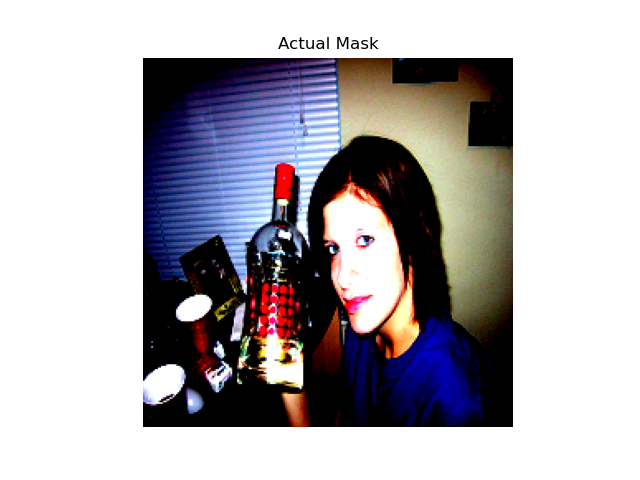
\includegraphics[width=0.8\textwidth]{include/plots/actual.png}
  \caption{Test Image}
  \label{fig:test_img}
\end{figure}




\subsection{Baseline Fully Convolutional Network}
For the baseline model, we trained the model with a learning rate of $1e^{-4}$ and a batch size of 16. It achieved a pixel accuracy of 0.704 and an IoU of 0.055 on the validation set, which as it is just a baseline, it only predicts black masks for all the images. Due to the fact that black is the most common class in the mask. But it serves as a good starting point for us to improve upon for this complex task.

The plots for the train and validation loss are, \hyperref[fig:baseline_train_loss]{here.}
And for the visualizations of the predicted mask, the actual mask and the actual mask over the predicted mask are \hyperref[fig:baseline_masks_visualization]{here.}

\begin{figure}[h!]
  \centering
  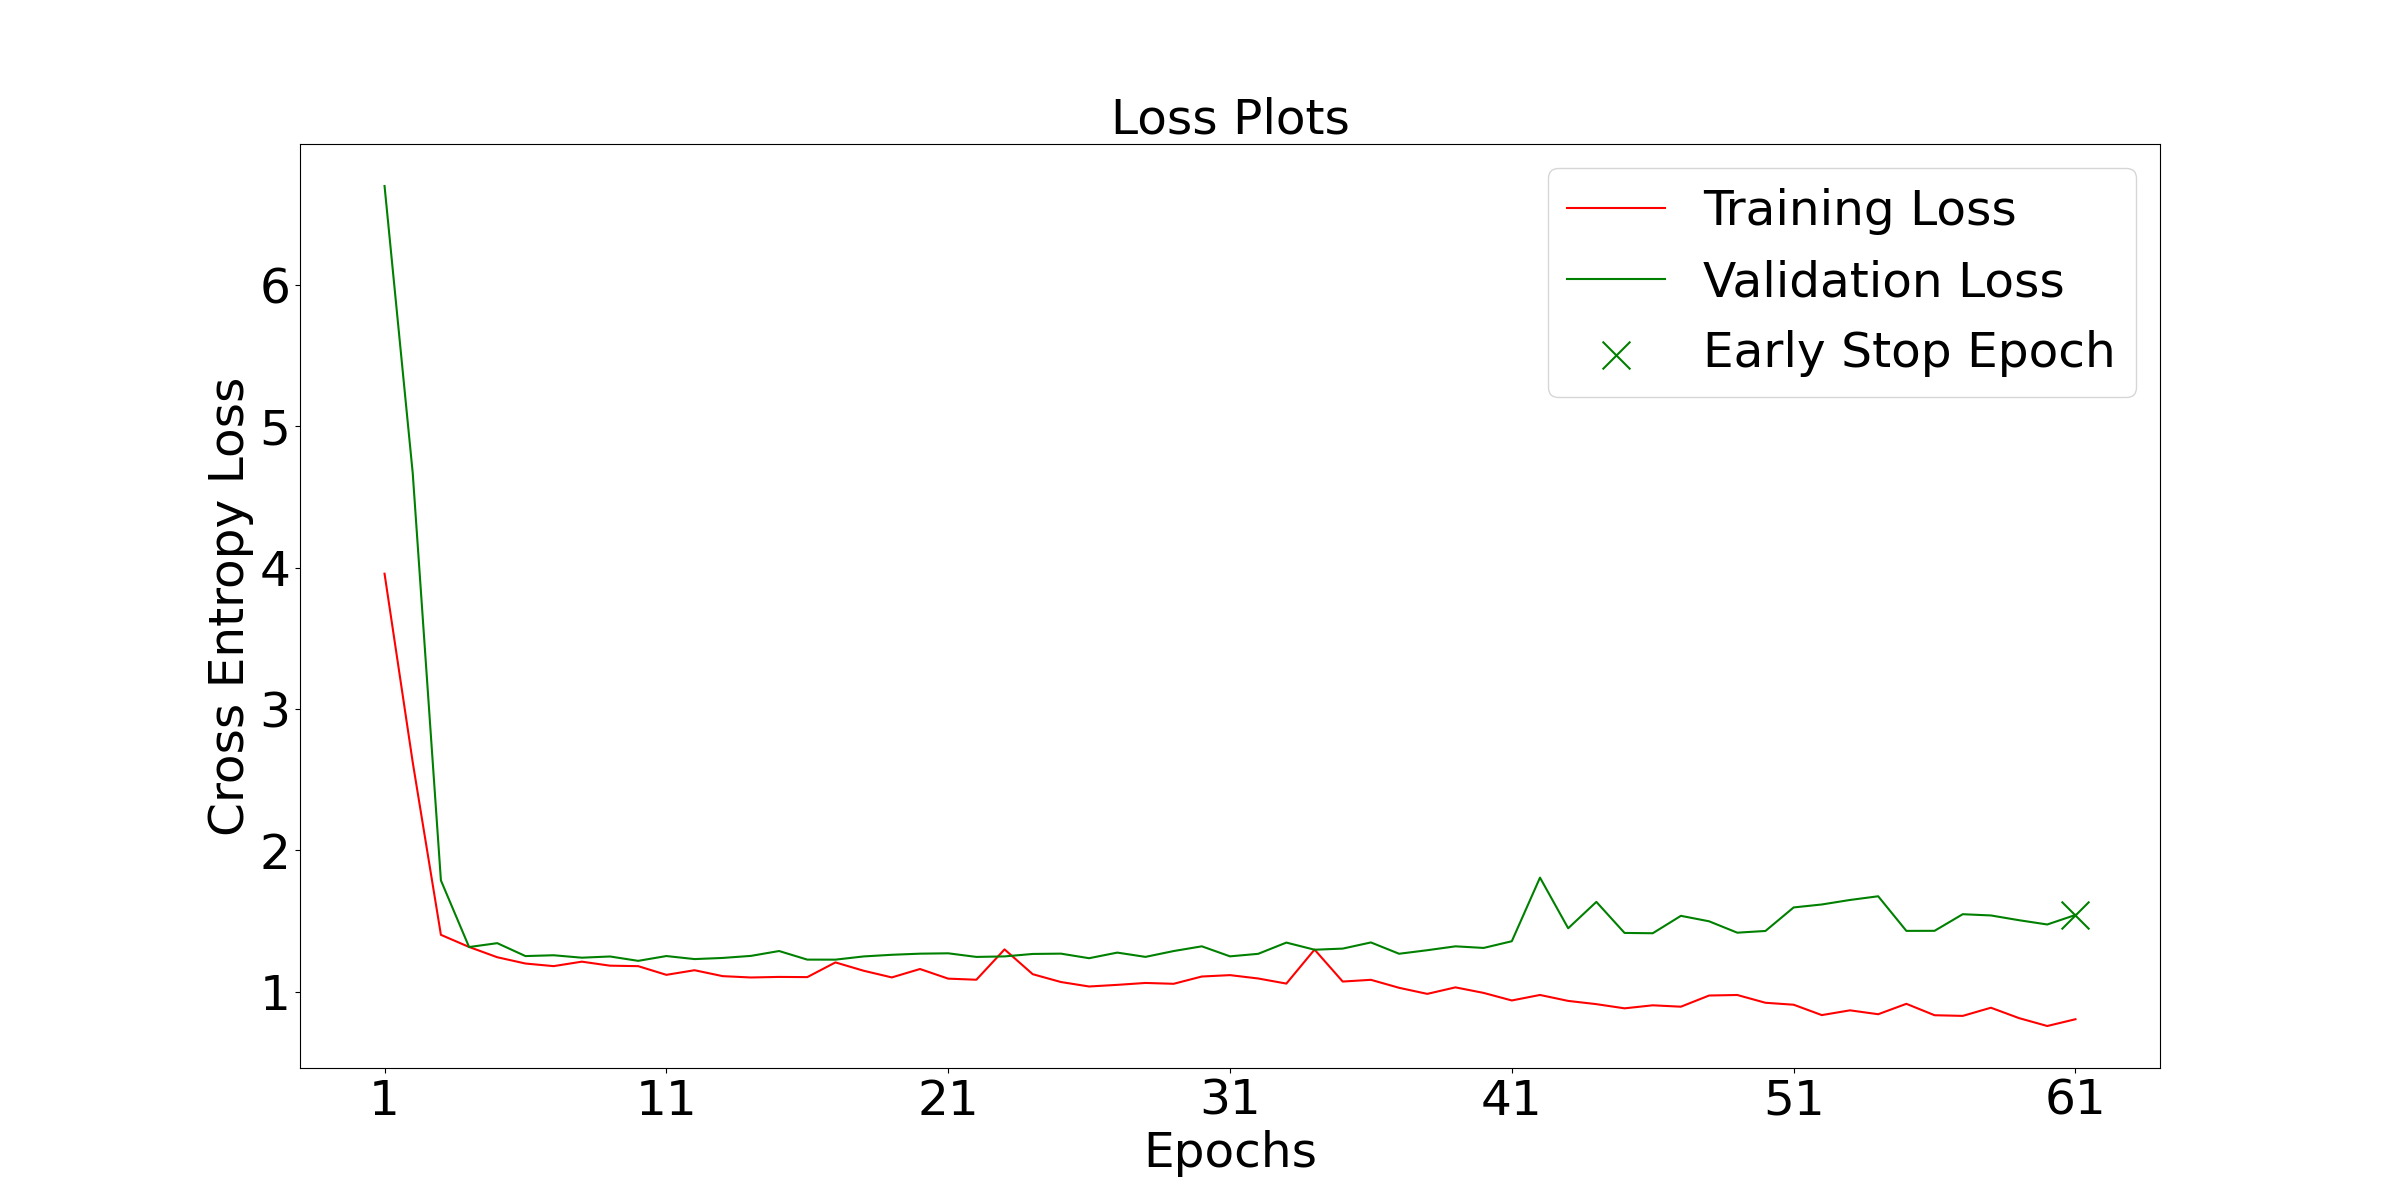
\includegraphics[width=0.8\textwidth]{include/plots/base_loss.png}
  \caption{Baseline Model Training/Validation Loss}
  \label{fig:baseline_train_loss}
\end{figure}

\begin{figure}[h!]
  \centering
  \begin{subfigure}[b]{0.45\textwidth}
      \centering
      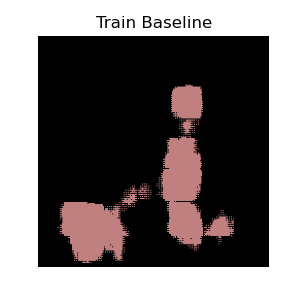
\includegraphics[width=\textwidth]{include/plots/base_pred.png}
      \caption{Baseline Model Prediction Mask}
      \label{fig:baseline_msk}
  \end{subfigure}
  \hfill %add desired spacing between images, e. g. ~, \quad, \qquad, \hfill etc. 
    %(or a blank line to force the subfigure onto a new line)
  \begin{subfigure}[b]{0.45\textwidth}
      \centering
      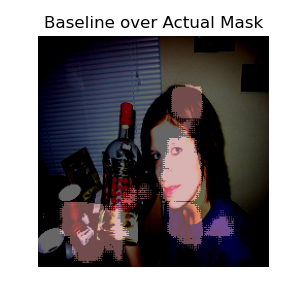
\includegraphics[width=\textwidth]{include/plots/baseline_over_actual.png} % Adjust width as needed
      \caption{Baseline Model Over Actual Mask}
      \label{fig:baseline_over_actual}
  \end{subfigure}
  \label{fig:baseline_masks_visualization}
\end{figure}

\subsection{Improvements on Baseline Model (Cosine Annealing Learning Rate)}
Using the same learning rate and batch size as the baseline model, we added the cosine annealing learning rate scheduler to the model. The model achieved an IoU of $0.0612$ and a pixel accuracy of $0.704$ on the validation set. The plots for the train and validation loss are, \hyperref[fig:cosine_annealing_train_loss]{here.} The visualizations of the predicted mask, the actual mask and the actual mask over the predicted mask are \hyperref[fig:cosine_annealing_masks_visualization]{here.}

\begin{figure}[h!]
  \centering
  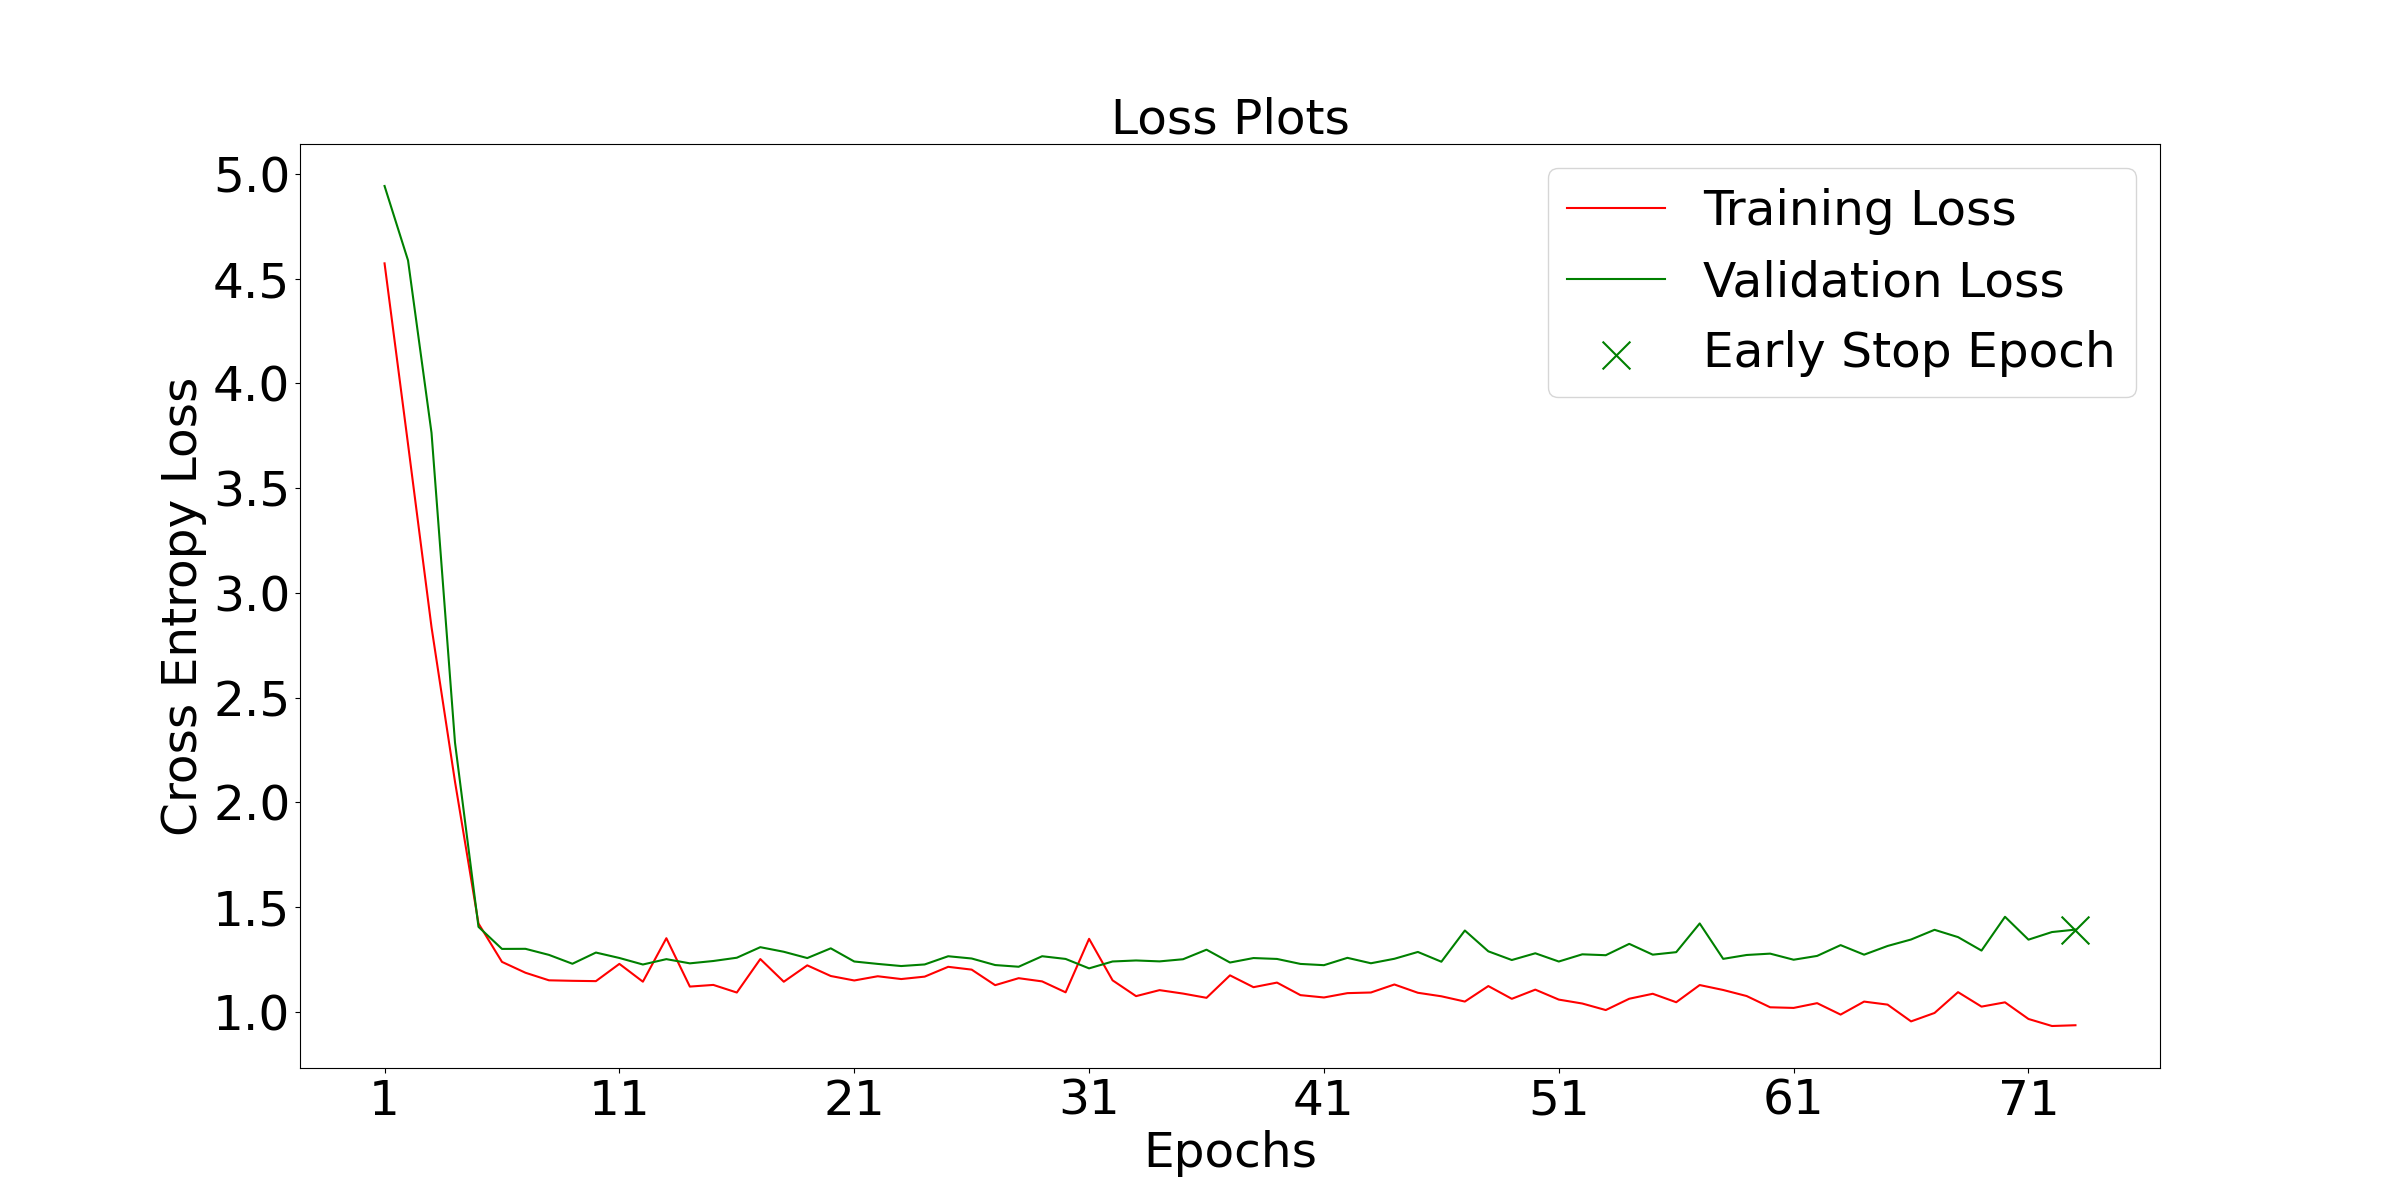
\includegraphics[width=0.8\textwidth]{include/plots/train_4_a_loss.png}
  \caption{Cosine Annealing Learning Rate Model Training/Validation Loss}
  \label{fig:cosine_annealing_train_loss}
\end{figure}

\begin{figure}[h!]
  \centering
  \begin{subfigure}[b]{0.45\textwidth}
      \centering
      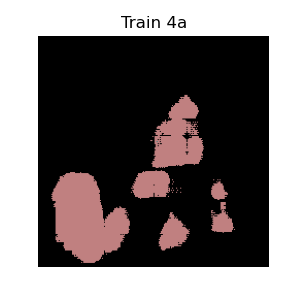
\includegraphics[width=\textwidth]{include/plots/train_4_a_pred.png}
      \caption{CosineAnnealingLR Model Prediction Mask}
      \label{fig:cosine_msk}
  \end{subfigure}
  \hfill %add desired spacing between images, e. g. ~, \quad, \qquad, \hfill etc. 
    %(or a blank line to force the subfigure onto a new line)
  \begin{subfigure}[b]{0.45\textwidth}
      \centering
      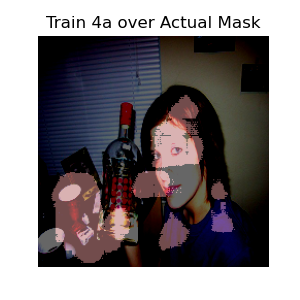
\includegraphics[width=\textwidth]{include/plots/train_4_a_over_actual.png} % Adjust width as needed
      \caption{CosineAnnealingLR Model Over Actual Mask}
      \label{fig:cosine_over_actual}
  \end{subfigure}
  \label{fig:cossine_annealing_masks_visualization}
\end{figure}

\subsection{Improvements on Baseline Model (Data Augmentation)}
Using the same learning rate and batch size as the baseline model, we added data augmentation and CosineAnnealingLR to the model. The model achieved an IoU of $0.0321$ and a pixel accuracy of $0.704$ on the validation set. The plots for the train and validation loss are, \hyperref[fig:data_augmentation_train_loss]{here.}

\begin{figure}[h!]
  \centering
  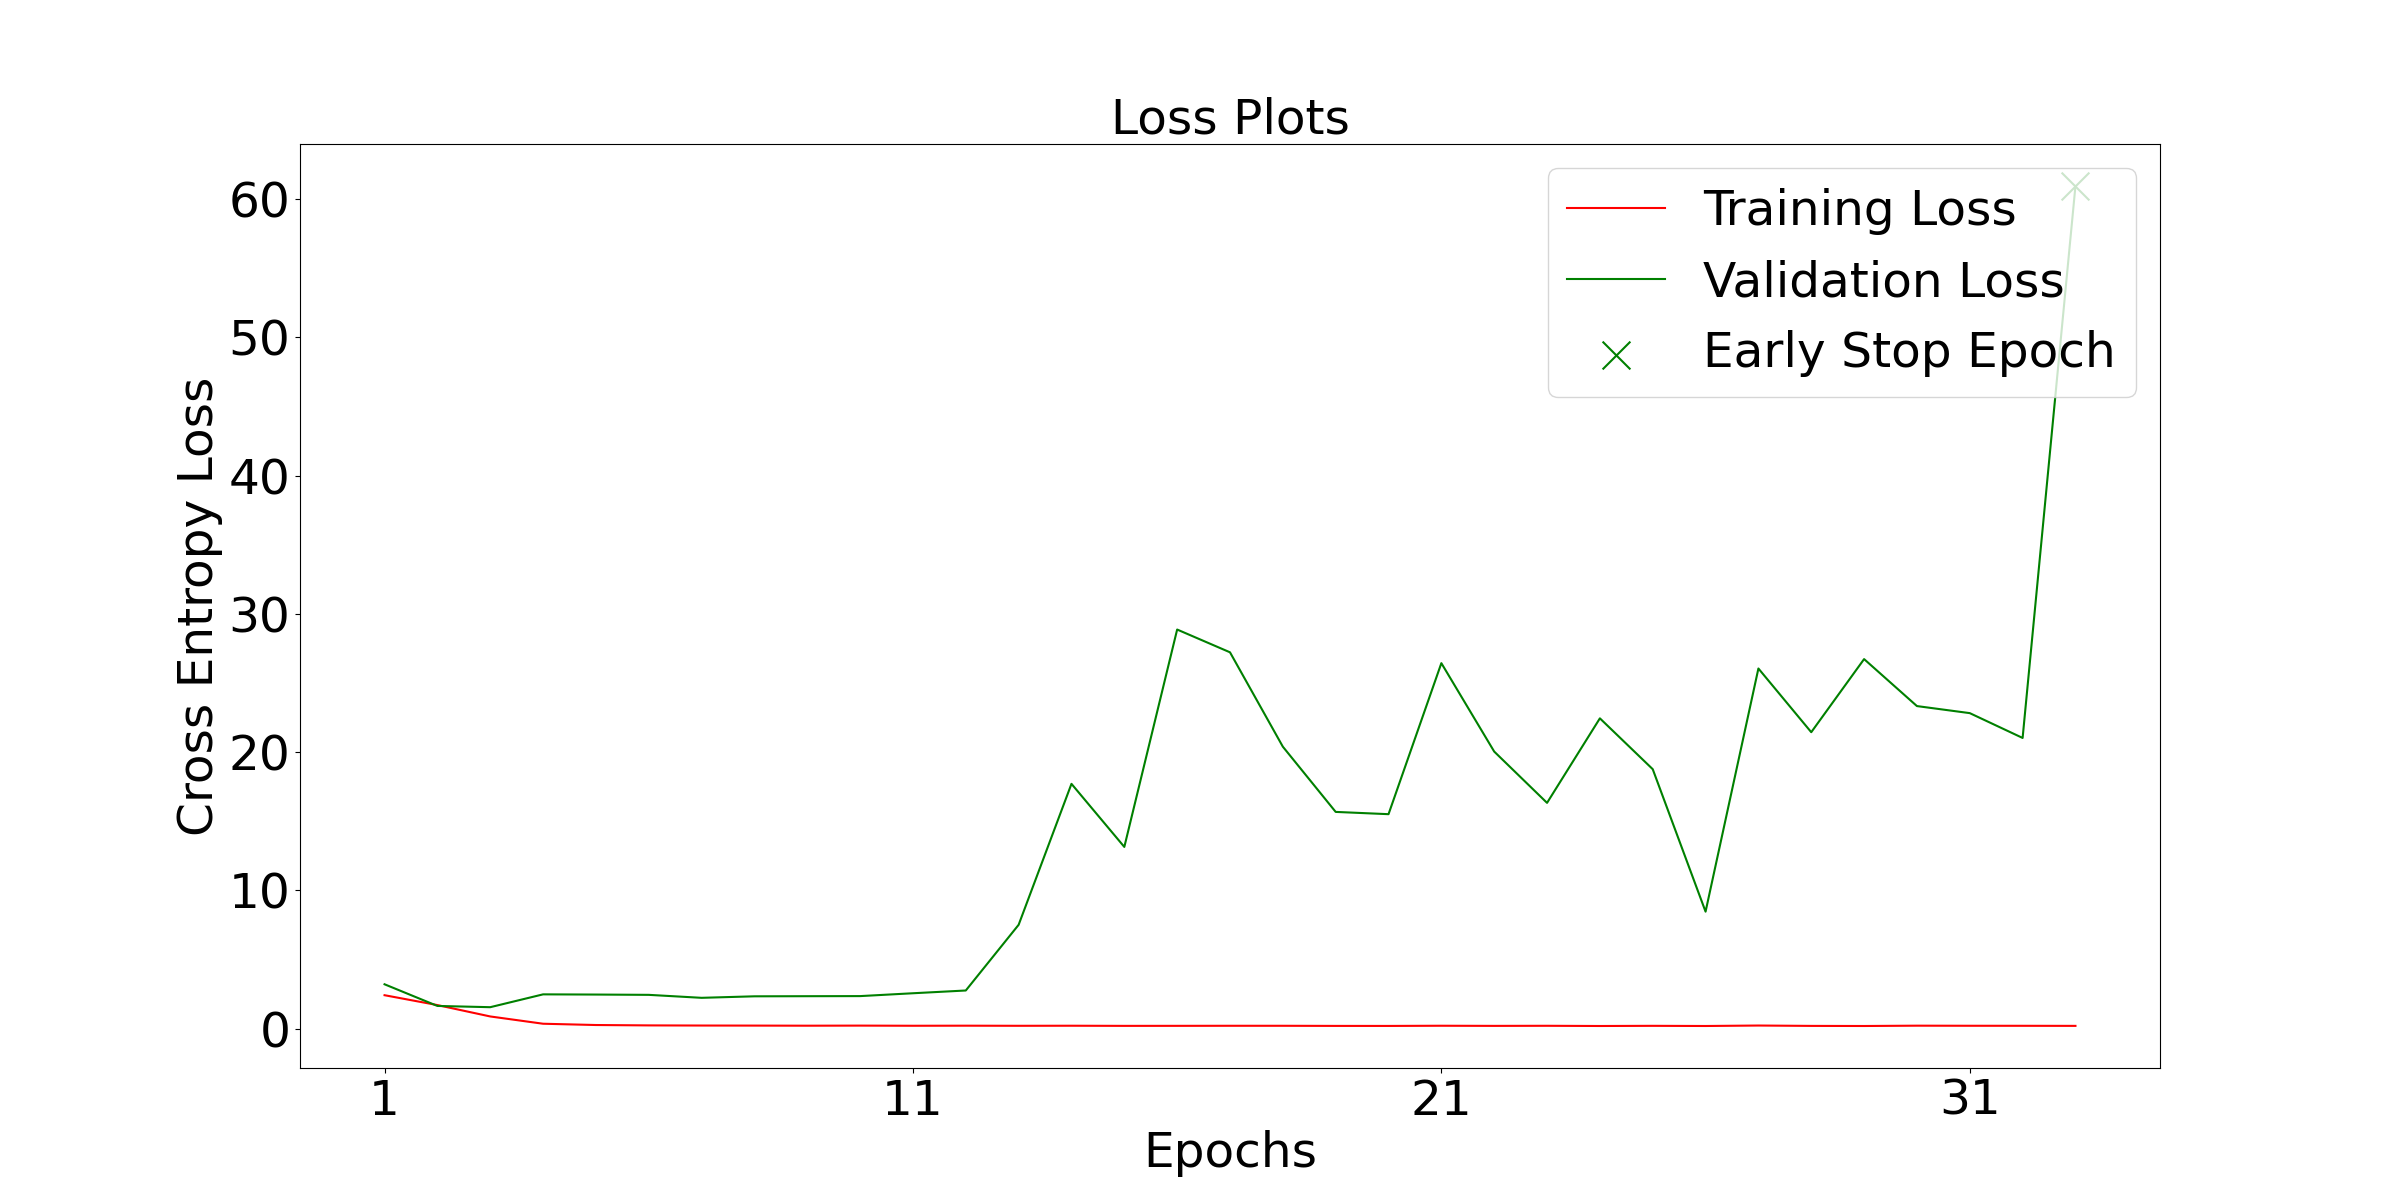
\includegraphics[width=0.8\textwidth]{include/plots/train_4_b_loss.png}
  \caption{Data Augmentation Model Training/Validation Loss}
  \label{fig:data_augmentation_train_loss}
\end{figure}

\begin{figure}[h!]
  \centering
  \begin{subfigure}[b]{0.45\textwidth}
      \centering
      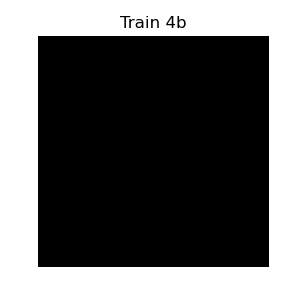
\includegraphics[width=\textwidth]{include/plots/train_4_b_pred.png}
      \caption{Data Augmentation Model Prediction Mask}
      \label{fig:data_augmentation_msk}
  \end{subfigure}
  \hfill %add desired spacing between images, e. g. ~, \quad, \qquad, \hfill etc. 
    %(or a blank line to force the subfigure onto a new line)
  \begin{subfigure}[b]{0.45\textwidth}
      \centering
      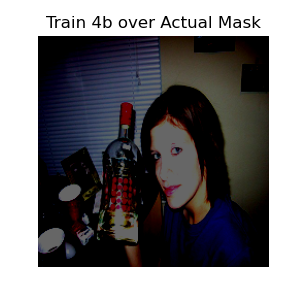
\includegraphics[width=\textwidth]{include/plots/train_4_b_over_actual.png} % Adjust width as needed
      \caption{Data Augmentation Model Over Actual Mask}
      \label{fig:data_augmentation_over_actual}
  \end{subfigure}
  \label{fig:data_augmentation_masks_visualization}
\end{figure}

\subsection{Improvements on Baseline Model (Class Imbalance)}
The last improvement we made to the baseline model was to implement a weighted loss criterion to fix the imbalanced classes issue. Using the same learning rate and batch size as the baseline model, we added the weighted loss criterion to the model. The model achieved an IoU of $0.0274$ and a pixel accuracy of $0.529$, The plots for the train and validation loss are, \hyperref[fig:weight_imbalanced_train_loss]{here.} The visualizations of the predicted mask, the actual mask and the actual mask over the predicted mask are \hyperref[fig:weight_imbalanced_masks_visualization]{here.}

\begin{figure}[h!]
  \centering
  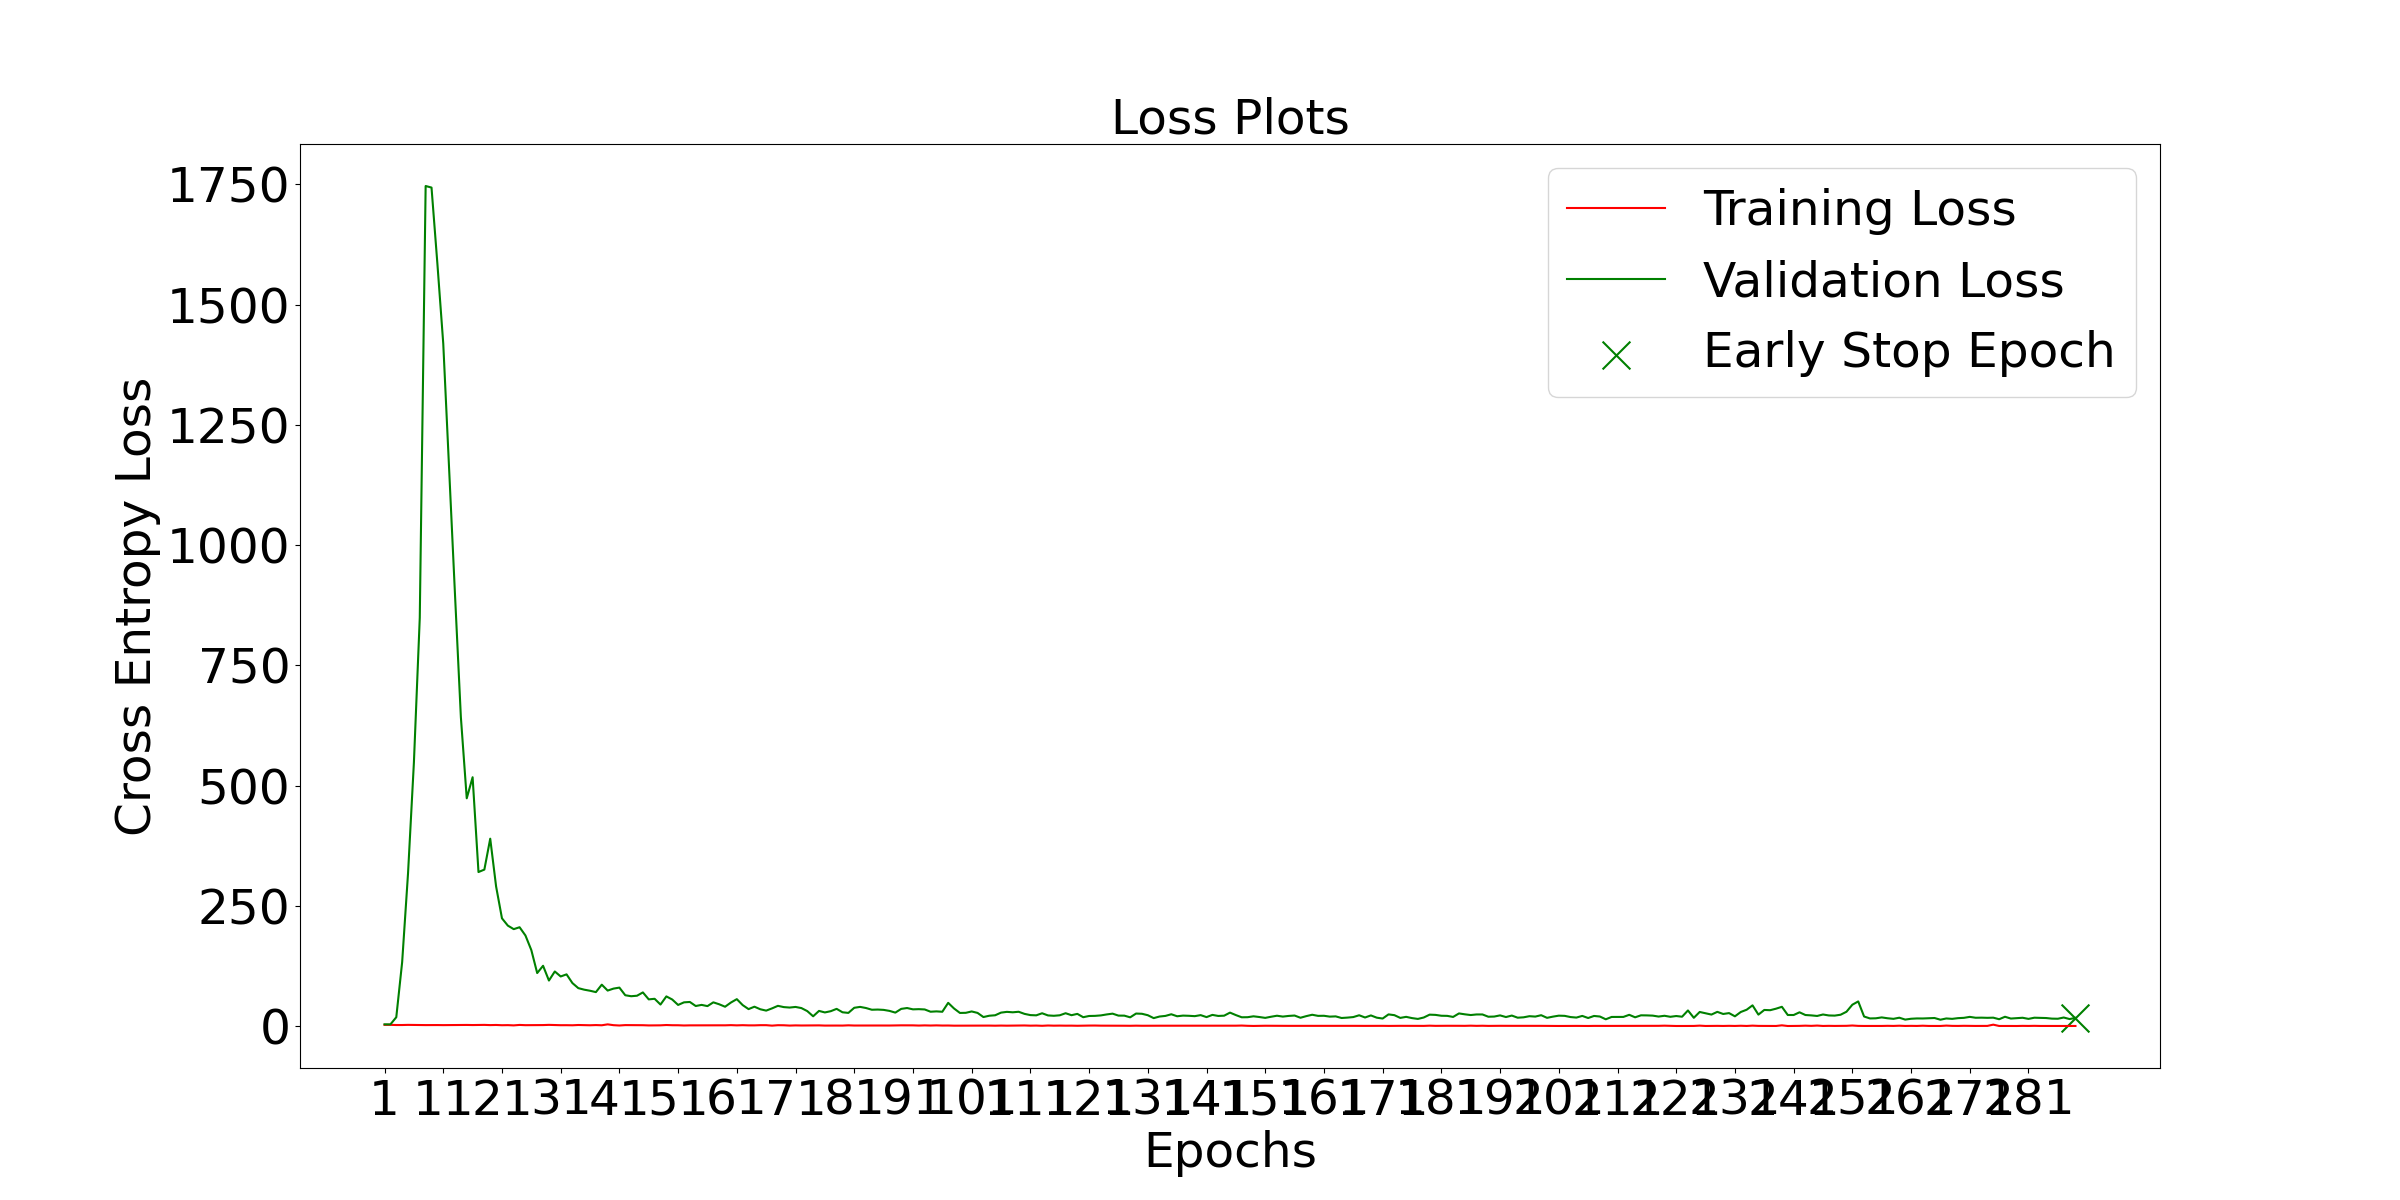
\includegraphics[width=0.8\textwidth]{include/plots/train_4_c_loss.png}
  \caption{Weighted Loss Criterion Model Training/Validation Loss}
  \label{fig:weight_imbalanced_train_loss}
\end{figure}

\begin{figure}[h!]
  \centering
  \begin{subfigure}[b]{0.45\textwidth}
      \centering
      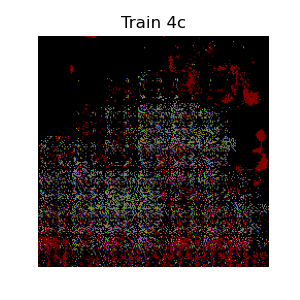
\includegraphics[width=\textwidth]{include/plots/train_4_c_pred.png}
      \caption{Weighted Loss Criterion Model Prediction Mask}
      \label{fig:weight_imbalanced_msk}
  \end{subfigure}
  \hfill %add desired spacing between images, e. g. ~, \quad, \qquad, \hfill etc. 
    %(or a blank line to force the subfigure onto a new line)
  \begin{subfigure}[b]{0.45\textwidth}
      \centering
      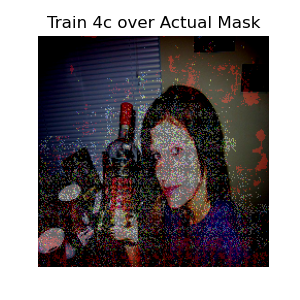
\includegraphics[width=\textwidth]{include/plots/train_4_c_over_actual.png} % Adjust width as needed
      \caption{Weighted Loss Criterion Model Over Actual Mask}
      \label{fig:weight_imbalanced_over_actual}
  \end{subfigure}
  \label{fig:weight_imbalanced_masks_visualization}
\end{figure}

\subsection{Custom FCN Architecture}
Using the same learning rate and batch size as the models from question 4, we trained the SimplifiedUNet model. Which achieved an IoU of $0.0383$ and a pixel accuracy of $0.751$ on the validation set. The plots for the train and validation loss are, \hyperref[fig:simplified_unet_train_loss]{here.} The visualizations of the predicted mask, the actual mask and the actual mask over the predicted mask are \hyperref[fig:simplified_unet_masks_visualization]{here.}

\begin{figure}[h!]
  \centering
  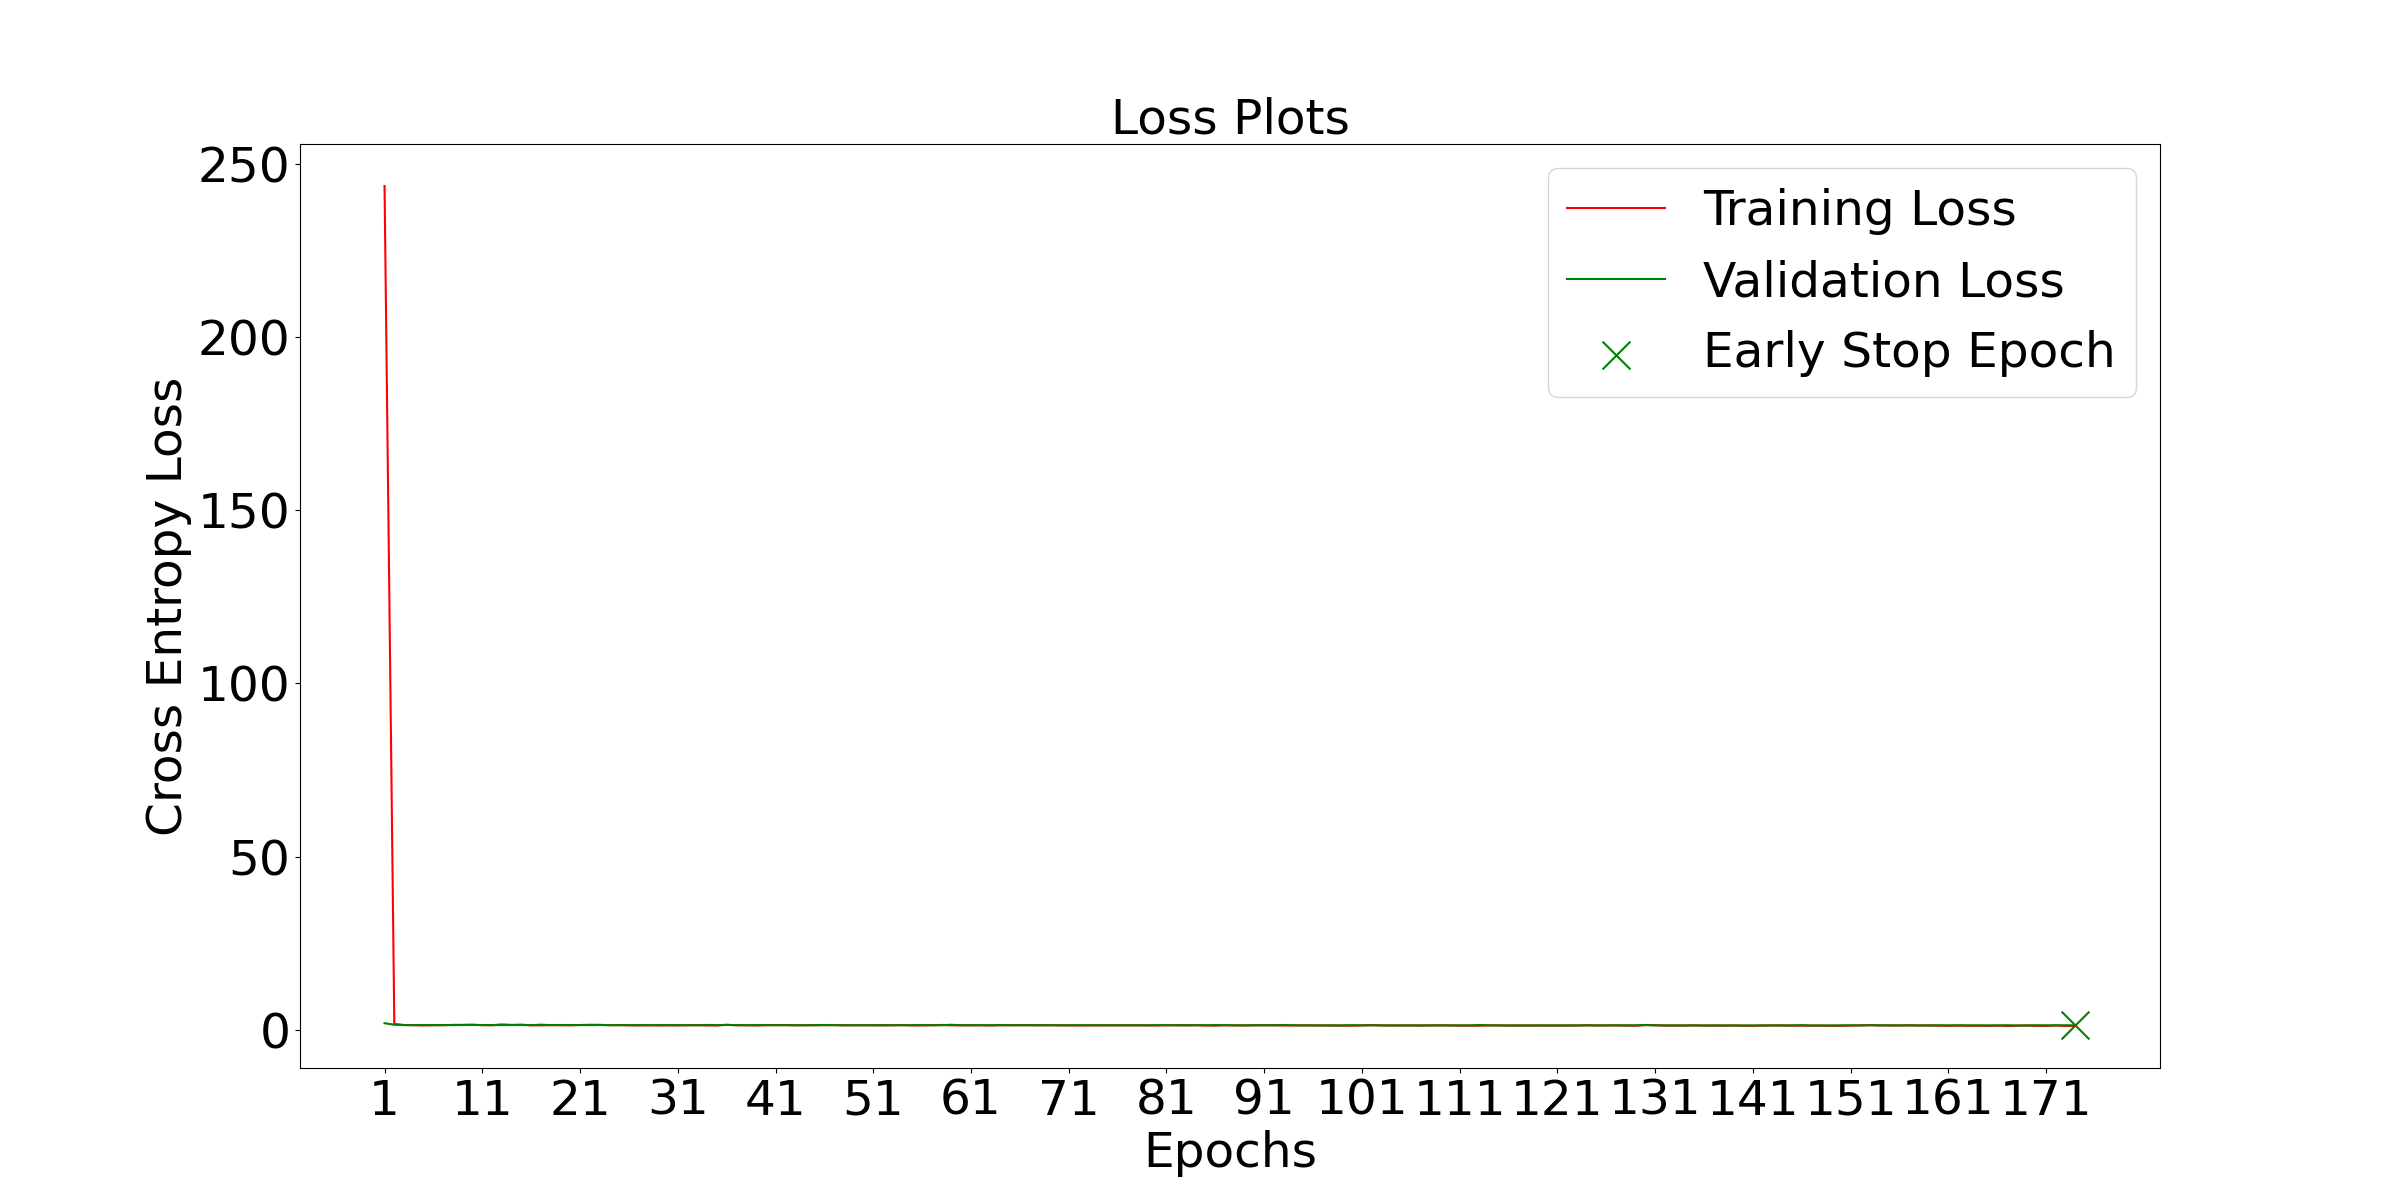
\includegraphics[width=0.8\textwidth]{include/plots/train_5_a_loss.png}
  \caption{Simplified UNet Model Training/Validation Loss}
  \label{fig:simplified_unet_train_loss}
\end{figure}

\begin{figure}[h!]
  \centering
  \begin{subfigure}[b]{0.45\textwidth}
      \centering
      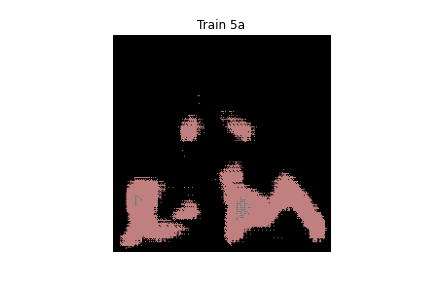
\includegraphics[width=\textwidth]{include/plots/train_5_a_pred.png}
      \caption{Simplified UNet Model Prediction Mask}
      \label{fig:simplified_unet_msk}
  \end{subfigure}
  \hfill %add desired spacing between images, e. g. ~, \quad, \qquad, \hfill etc. 
    %(or a blank line to force the subfigure onto a new line)
  \begin{subfigure}[b]{0.45\textwidth}
      \centering
      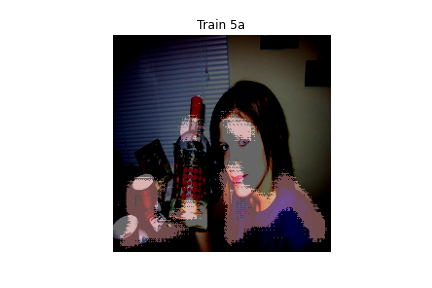
\includegraphics[width=\textwidth]{include/plots/train_5_a_over_actual.png} % Adjust width as needed
      \caption{Simplified UNet Model Over Actual Mask}
      \label{fig:simplified_unet_over_actual}
  \end{subfigure}
  \label{fig:simplified_unet_masks_visualization}
\end{figure}


\subsection{ResNet-50}
Using the same learning rate and batch size as the models from question 4, we used a pretrained model from pytorch which was the resnet50 model. The model achieved an IoU of $0.157$ and a pixel accuracy of $0.824$ on the validation set. The plots for the train and validation loss are, \hyperref[fig:resnet50_train_loss]{here.} The visualizations of the predicted mask, the actual mask and the actual mask over the predicted mask are \hyperref[fig:resnet50_masks_visualization]{here.}

\begin{figure}[h!]
  \centering
  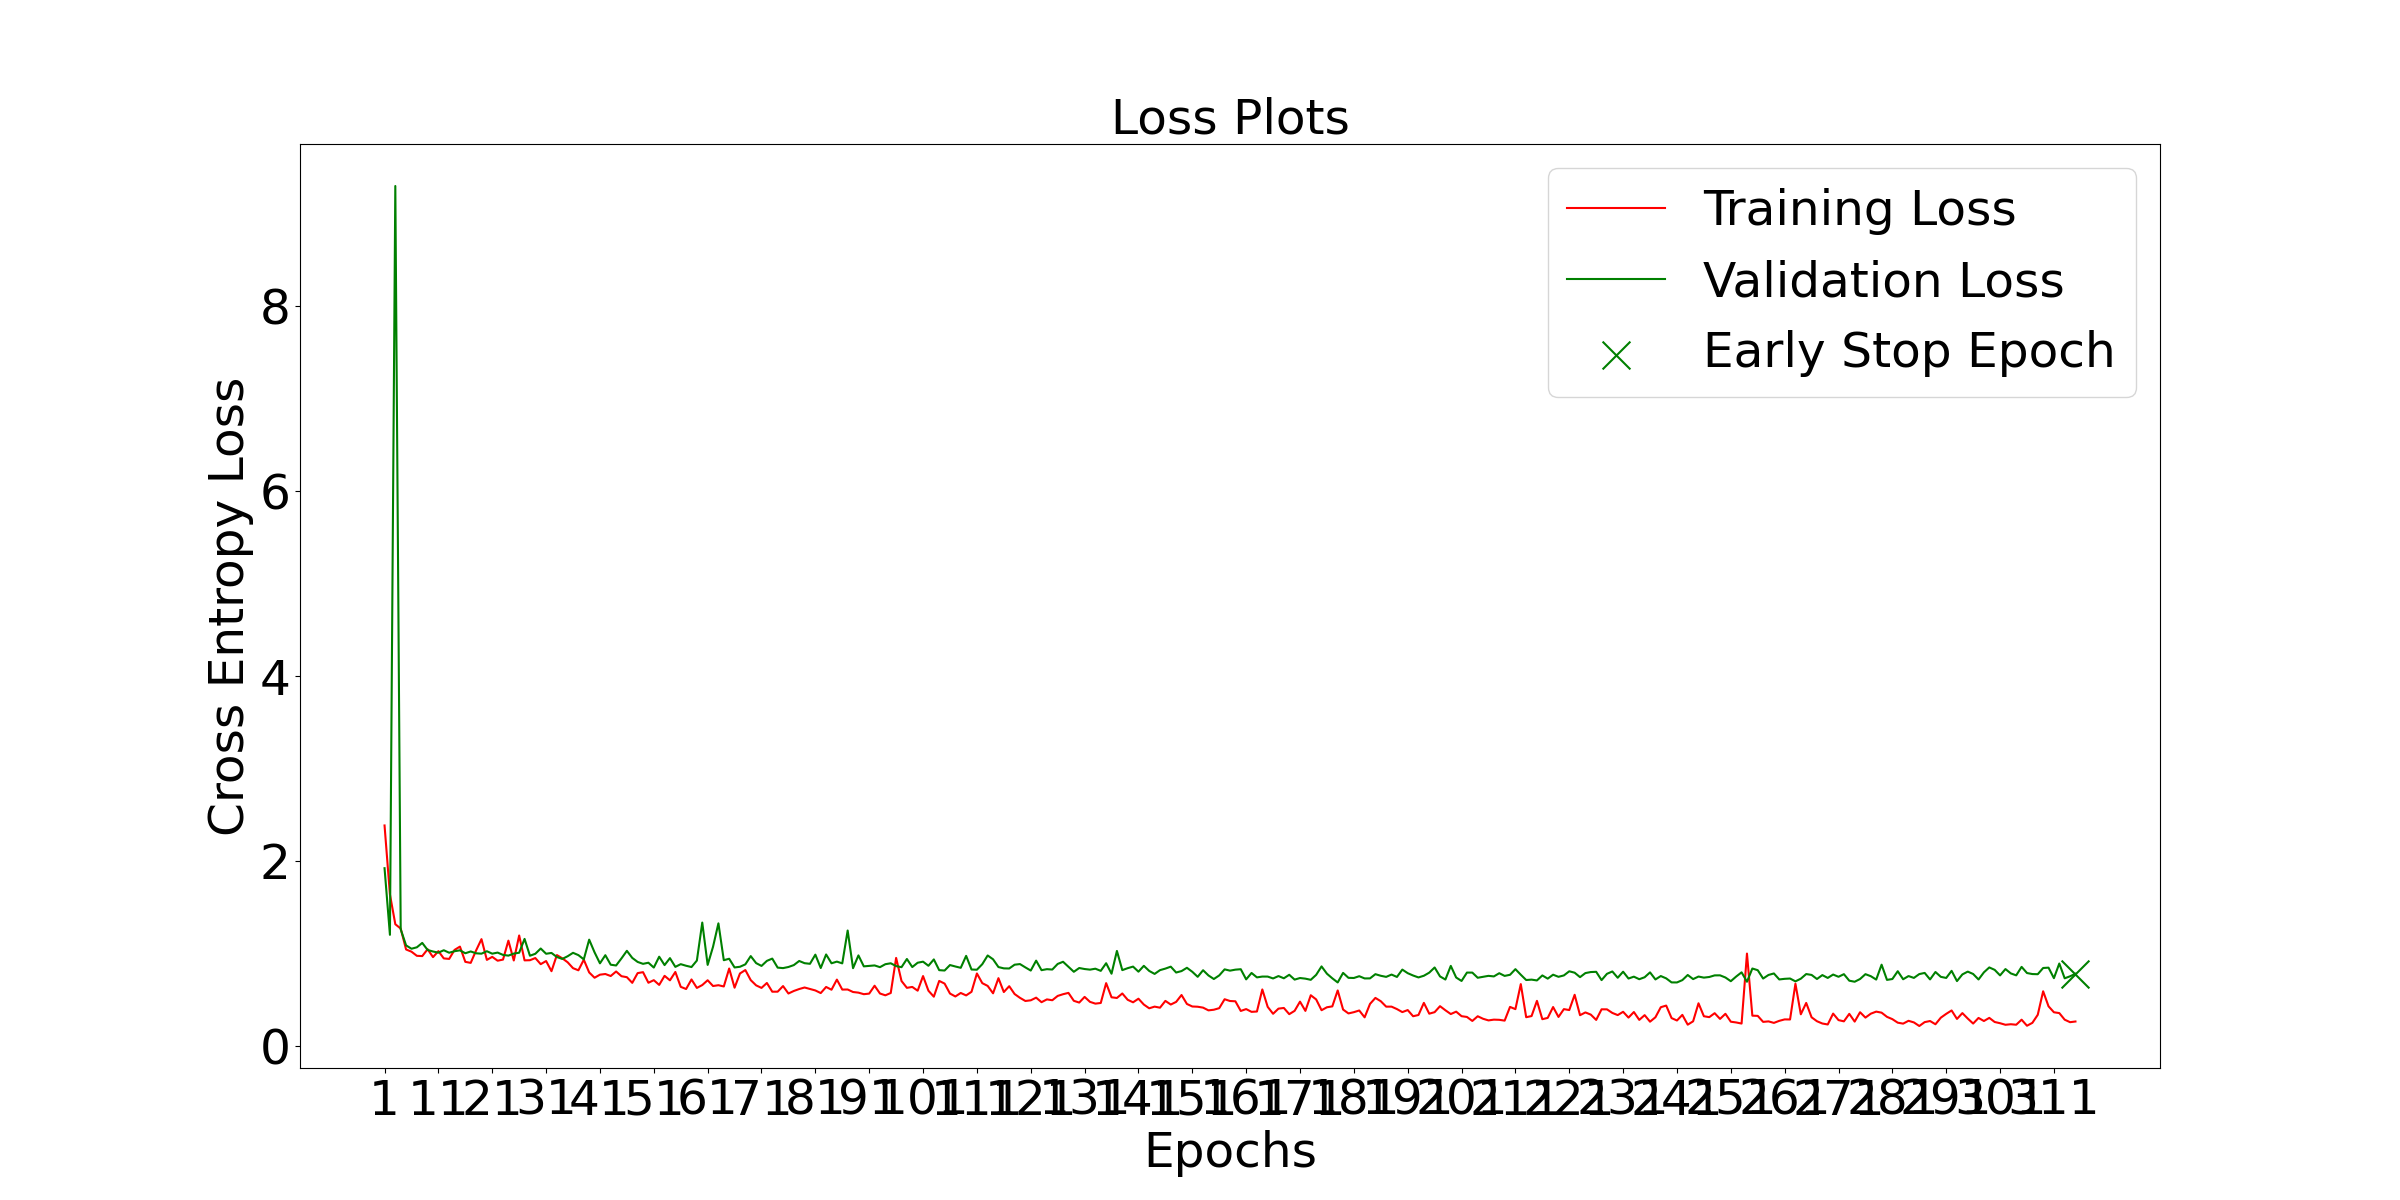
\includegraphics[width=0.8\textwidth]{include/plots/train_5_b_loss.png}
  \caption{ResNet-50 Model Training/Validation Loss}
  \label{fig:resnet50_train_loss}
\end{figure}

\begin{figure}[h!]
  \centering
  \begin{subfigure}[b]{0.45\textwidth}
      \centering
      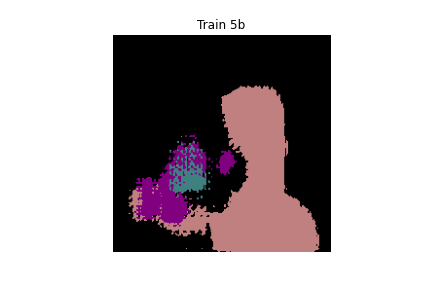
\includegraphics[width=\textwidth]{include/plots/train_5_b_pred.png}
      \caption{ResNet-50 Model Prediction Mask}
      \label{fig:resnet50_msk}
  \end{subfigure}
  \hfill %add desired spacing between images, e. g. ~, \quad, \qquad, \hfill etc. 
    %(or a blank line to force the subfigure onto a new line)
  \begin{subfigure}[b]{0.45\textwidth}
      \centering
      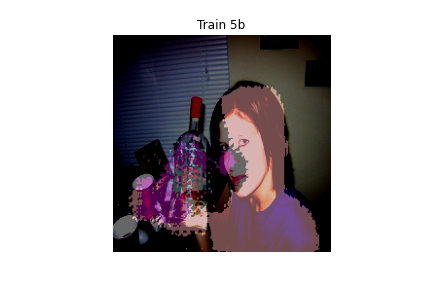
\includegraphics[width=\textwidth]{include/plots/train_5_b_over_actual.png} % Adjust width as needed
      \caption{ResNet-50 Model Over Actual Mask}
      \label{fig:resnet50_over_actual}
  \end{subfigure}
  \label{fig:resnet50_masks_visualization}
\end{figure}

\subsection{U-Net}
For the U-Net model, we trained using the same learning rate and batch size as the models from question 4. The model achieved an IoU of $0.0358$ and a pixel accuracy of $0.751$ on the validation set. The plots for the train and validation loss are, \hyperref[fig:unet_train_loss]{here.} The visualizations of the predicted mask, the actual mask and the actual mask over the predicted mask are \hyperref[fig:unet_masks_visualization]{here.}

\begin{figure}[h!]
  \centering
  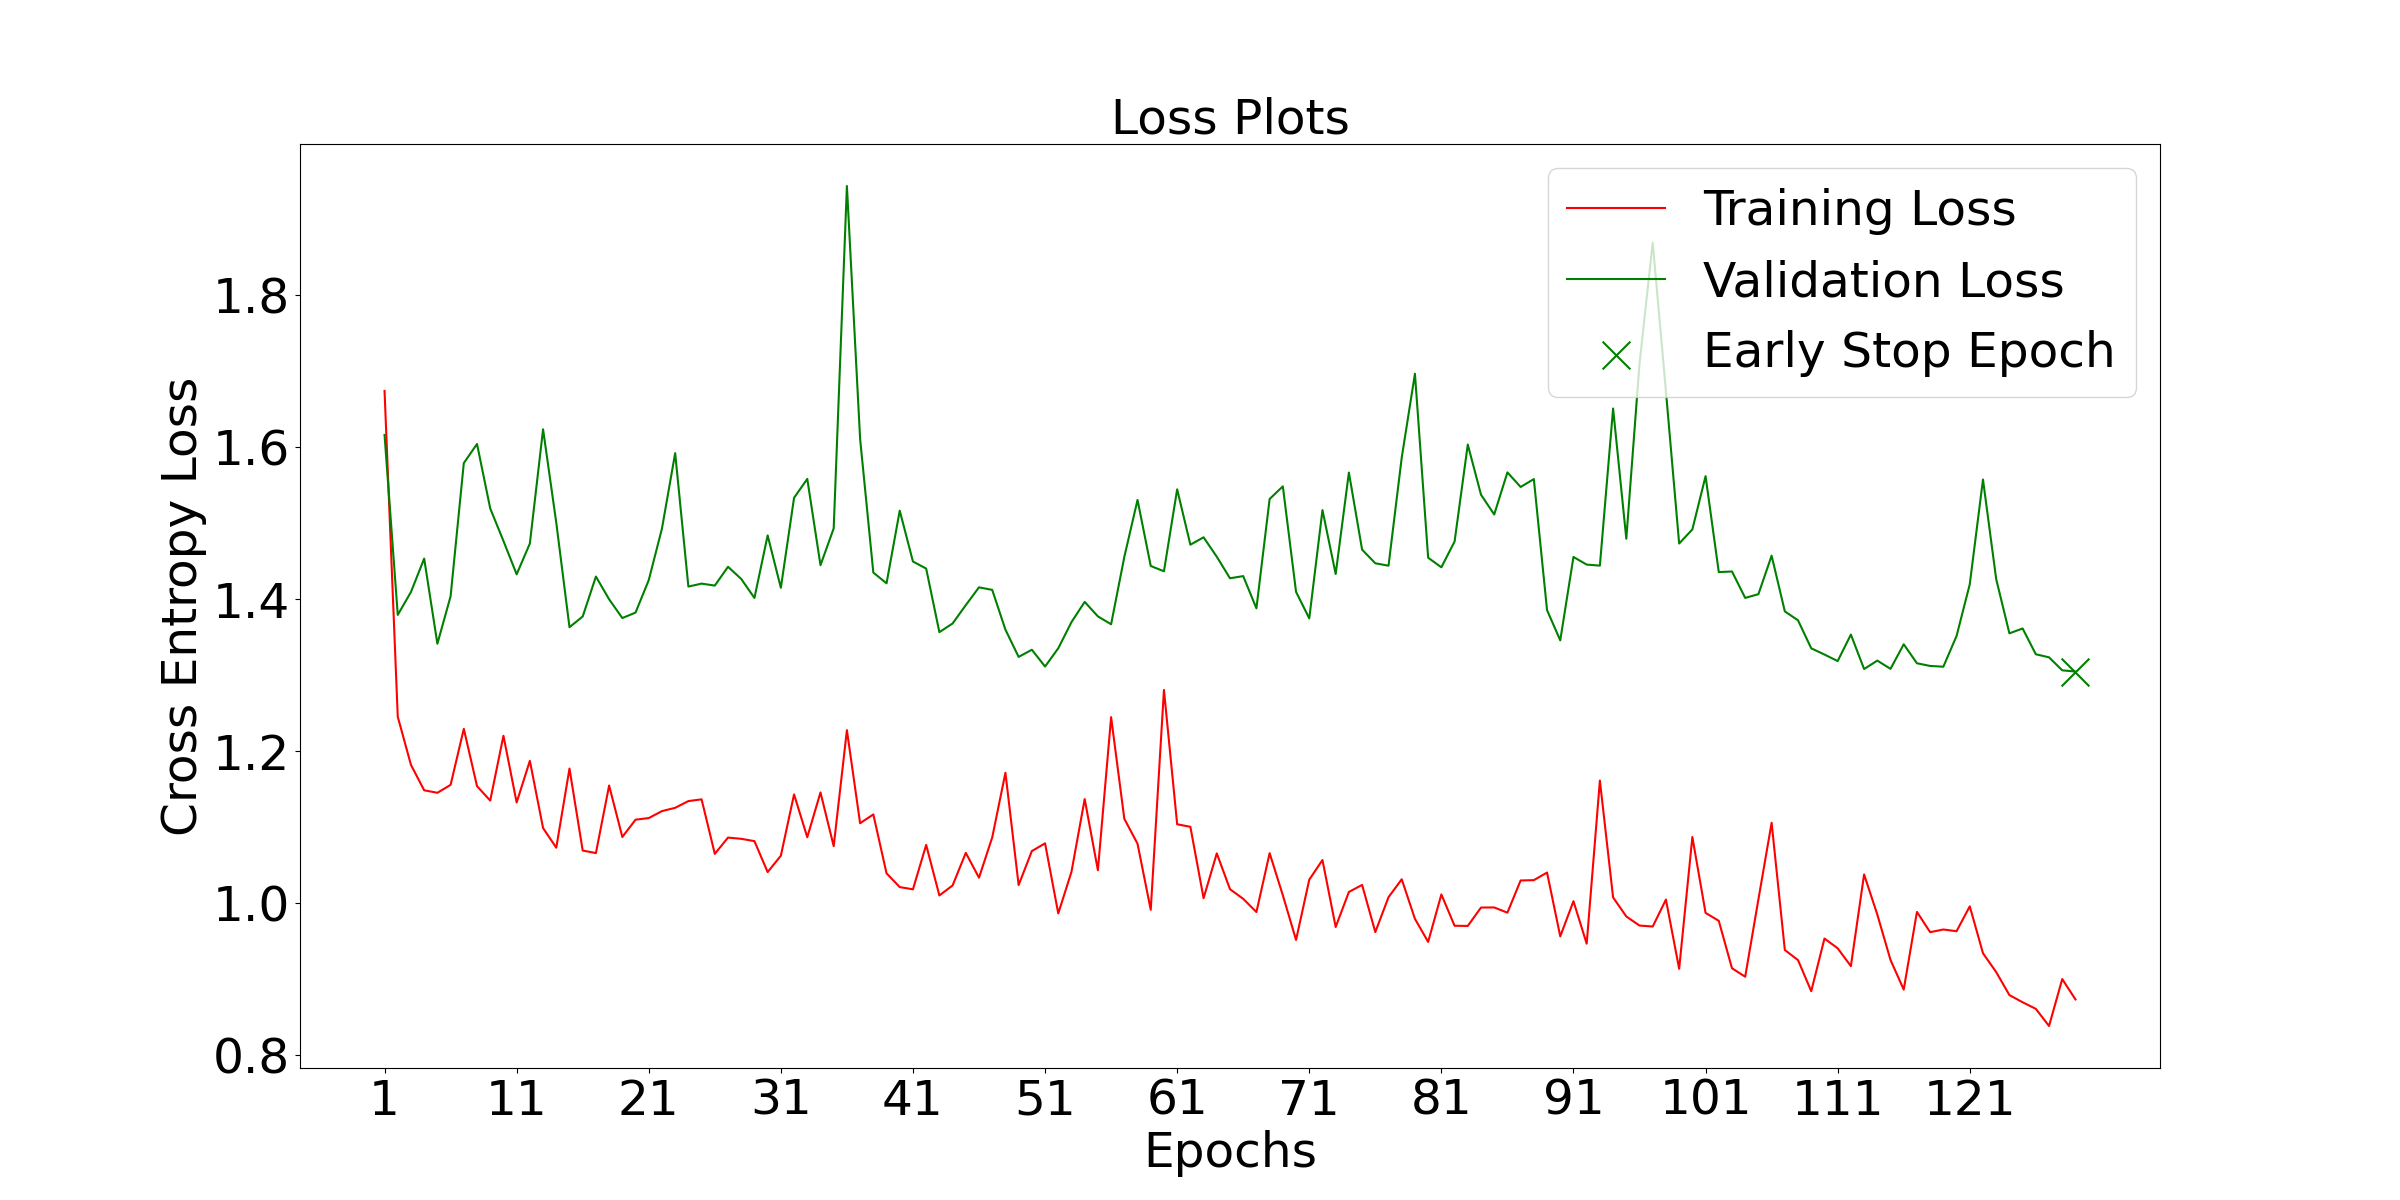
\includegraphics[width=0.8\textwidth]{include/plots/train_5_c_loss.png}
  \caption{U-Net Model Training/Validation Loss}
  \label{fig:unet_train_loss}
\end{figure}

\begin{figure}[h!]
  \centering
  \begin{subfigure}[b]{0.45\textwidth}
      \centering
      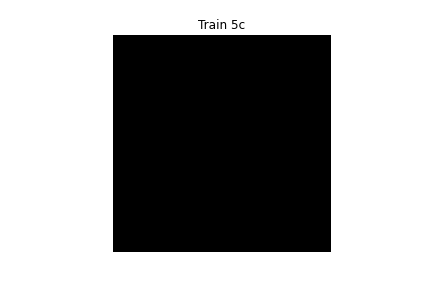
\includegraphics[width=\textwidth]{include/plots/train_5_c_pred.png}
      \caption{U-Net Model Prediction Mask}
      \label{fig:unet_msk}
  \end{subfigure}
  \hfill %add desired spacing between images, e. g. ~, \quad, \qquad, \hfill etc. 
    %(or a blank line to force the subfigure onto a new line)
  \begin{subfigure}[b]{0.45\textwidth}
      \centering
      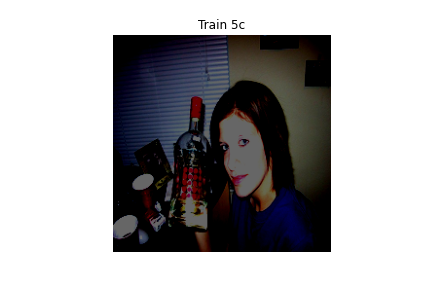
\includegraphics[width=\textwidth]{include/plots/train_5_c_over_actual.png} % Adjust width as needed
      \caption{U-Net Model Over Actual Mask}
      \label{fig:unet_over_actual}
  \end{subfigure}
  \label{fig:unet_masks_visualization}
\end{figure}

We did however, have a better run with the U-Net with the exact same parameters on a previous run, but for some reason we are unable to replicate the same results, we did not record down the IoU but we have the image you see \hyperref[fig:unet_best_run]{below} which is the best run we had with the U-Net model as it was able to make the outline of the bird in the image.

\begin{figure}[h!]
  \centering
  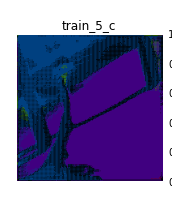
\includegraphics[width=0.7\textwidth]{include/plots/better_5c.png}
  \caption{U-Net Model Best Run Prediction Mask}
  \label{fig:unet_best_run}
\end{figure}
\newpage
\section{Discussion}

\subsection{Baseline Fully Convolutional Network}
In our baseline implementation, many decisions were made regarding loss criterion, learning rate, and model architecture. For instance, using Cross Entropy Loss as the loss function was utilized for our task due to its appropriateness for multi-class classification problems, such as semantic segmentation on diverse object categories. Additionally, using FCN architecture and Xavier initialization addressed the challenge of weight initialization in deep neural networks, such as preventing vanishing or exploding gradients and balancing between the weight's scale and input's data scale. This allows us to have a more stable training process to use as a foundation for experimentation and improvements later. As a result, our IoU and accuracy were somewhat decent with our baseline detecting the general location of some objects in the images. For instance, in our example image, our baseline was able to identify the woman as human and located the general location of her head and hand.

However, given it's a baseline model, there are many drawbacks. For one, the absence of a learning rate schedule poses as a limitation due to unpredictable and suboptimal convergence dynamics. Furthermore, we did not implement class imbalance which is critical for segmentation. When classes are imbalanced, that class or some classes may dominate the image, while some other classes make up only a small portion of the image. This means the network can reduce the error considerably just by labeling everything with the majority class. Consequently, our IoU and accuracy were relatively low. As seen in the example image, our baseline was only able to classify the human and no other object, labeling the rest as background. Additionally, the overall shape of the human was generally vague and indistinguishable.
\subsection{Improvements on Baseline Model}
Several key approaches were made to improve the overall model of the performance, including cosine annealing learning rate scheduler, applying transformations to the input images and labels, and addressing the rare class/imbalanced class problem. Firstly, implementing cosine annealing improved the convergence by dynamically adjusting the learning rate during training, speeding convergence and avoiding overshooting or getting  stuck in high-loss regions. Additionally, including transformers in the architecture and randomizing them prevents overfitting, especially where contextual information may play a role. Addressing the class imbalance problem prevents the model from exhibiting bias toward dominant classes, encouraging the model to correctly classify minority classes and generalize better results. 

However, with fine-tuning to the baseline model comes with problems such as hyperparameter sensitivity . Both cosine annealing and class balancing involve hyperparameters that require tuning such as T\_max and eta\_min in cosine annealing and our current choices may not be effective for our training process. Furthermore, class balancing can be sensitive to the choice of class weights and suboptimal weights may not fully address the class imbalance issue. As a result of these improvements and their drawbacks, our IoU and pixel accuracy increased but not as substantially as we expected. From the example image, you can see that the model was able to correctly classify the woman as human and with more precision than the base model, but the model still was only able to detect one type of object.

\subsection{Expirements with other architectures}
In our experimentation models (simplified UNET, Transfer Learning with a ResNet Encoder, UNET), there were improvements from the improved baseline model. We reused all of the improvements we created in question 4 in all of the models above, and we used the same parameters (ie learning rate, weight initialization) as before. These models improved our performance from the last section. Using transfer learning with a ResNet34 encoder to improve an FCN architecture made performance better because this type of model has better feature extraction in the encoder due to ResNet34 being pretraining on ImageNet, which provides a regularization effect. Also, it leads to a faster initial convergence, for it only trains the decoder first while leveraging pre-extracted features. UNET improves performance compared to an FCN because in the UNET decoder, the encoder provides a large number of feature channels to each upsampled layer, so the model is able to maintain contextual information in these channels. Furthermore, UNET has more precise and spatially coherent segmentations due to the architecture consisting of a contracting path to capture context and a symmetric expanding path that enables precise localization.

However, as seen on the graphs, UNET did not perform exactly the way we wanted it to. When we tried to train UNET with our current python file, it quickly converges and produces a completely black mask, but in one run before, we had one to perfectly trace out every object of the image, but classifying all of it wrong. 
UNET works better with HE weight initializations, but we used the Xavier weight initializations, which may have caused it to converge to a black mask most of our runs. Even though it had satisfactory, using transfer learning with a ResNet34 encoder into an FCN did come with some consequences. Specifically, the ResNet34 encoder has significantly more layers and latency compared to a simple fully convolutional encoder because it is a large encoder, so it lead to a longer training time as shown by the number of epochs.

\subsection{IoU Implementation difference}
We tested the training with an initially unmodified IoU which would take the entire image class IoU by each individual image in the batch. This produced a good baseline IoU of 0.05, and changed increasingly with our different improvements up to an IoU of 0.075 at the end. However, we found this method of storing the best models ineffective, as the visualizations we were seeing were at most times either completely black or noisy.

After changing our IoU to not producing the means per image, but instead first individually averaging over by the class for all images in the batch, then only aggregated to a total mean, we find that this metric, despite having obviously lower values, was able to qualitatively produce better visualizations observed in the returned image masks. Because of this, our IoUs are seemingly small, but their associated best models perform observably better. This is reflected in our transfer training with ResNet50 which was our best performing model, achieving a mean IoU of 0.157 even with this new metric.


\newpage
\section{Best Model}
From all the models that we trained above, the best performing model that we got was the ResNet-50 model. It achieved an IoU of $0.157$ and a pixel accuracy of $0.824$ on the validation set. 

Here are some plots and example on other images that worked extremely well with the ResNet-50 model.

\begin{figure}[h]
  \centering
  \begin{subfigure}[b]{0.45\textwidth}
      \centering
      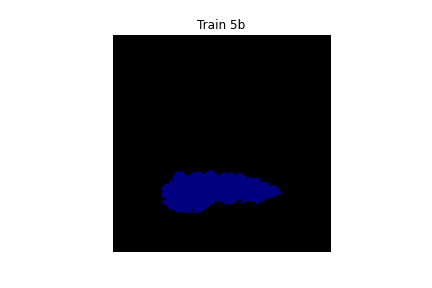
\includegraphics[width=\textwidth]{include/best model/boat1_pred.png}
      \caption{Boat Prediction Mask}
  \end{subfigure}
  \hfill %add desired spacing between images, e. g. ~, \quad, \qquad, \hfill etc. 
    %(or a blank line to force the subfigure onto a new line)
  \begin{subfigure}[b]{0.45\textwidth}
      \centering
      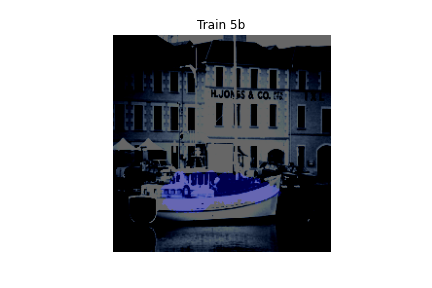
\includegraphics[width=\textwidth]{include/best model/boat1_over_actual.png} % Adjust width as needed
      \caption{Boat Over Actual Mask}
  \end{subfigure}
  \begin{subfigure}[b]{0.45\textwidth}
    \centering
    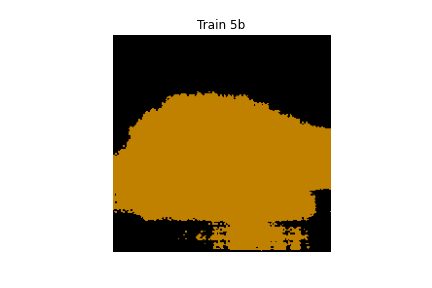
\includegraphics[width=\textwidth]{include/best model/dinningtable1_pred.png}
    \caption{Dinning Table Prediction Mask}
\end{subfigure}
\hfill %add desired spacing between images, e. g. ~, \quad, \qquad, \hfill etc. 
  %(or a blank line to force the subfigure onto a new line)
\begin{subfigure}[b]{0.45\textwidth}
    \centering
    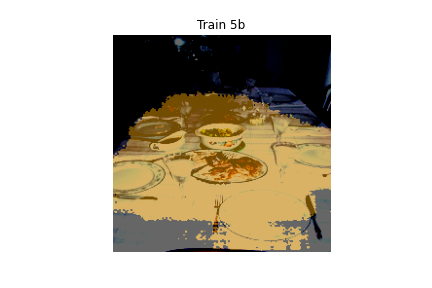
\includegraphics[width=\textwidth]{include/best model/diningtable1_over_actual.png} % Adjust width as needed
    \caption{Dinning Table Over Actual Mask}
\end{subfigure}
\begin{subfigure}[b]{0.45\textwidth}
  \centering
  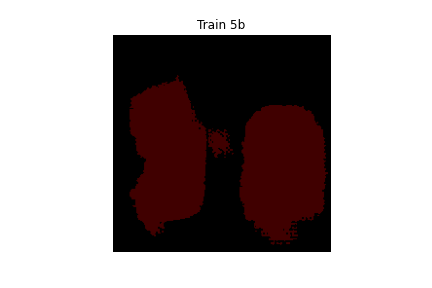
\includegraphics[width=\textwidth]{include/best model/cat1_pred.png}
  \caption{Cat Prediction Mask}
\end{subfigure}
\hfill %add desired spacing between images, e. g. ~, \quad, \qquad, \hfill etc. 
%(or a blank line to force the subfigure onto a new line)
\begin{subfigure}[b]{0.45\textwidth}
  \centering
  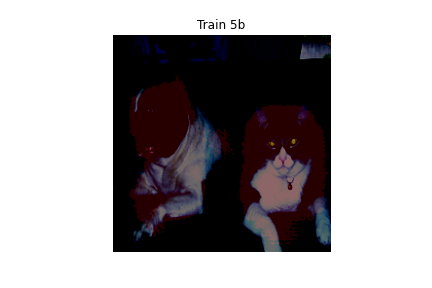
\includegraphics[width=\textwidth]{include/best model/cat1_over_actual.png} % Adjust width as needed
  \caption{Cat Over Actual Mask}
\end{subfigure}
  \label{fig:best_models1}
\end{figure}

\begin{figure}[h]
  \begin{subfigure}[b]{0.45\textwidth}
    \centering
    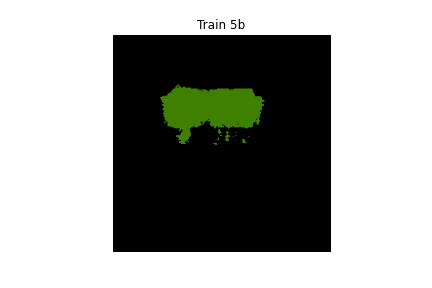
\includegraphics[width=\textwidth]{include/best model/cow1_pred.png}
    \caption{Cow Prediction Mask}
  \end{subfigure}
  \hfill %add desired spacing between images, e. g. ~, \quad, \qquad, \hfill etc. 
  %(or a blank line to force the subfigure onto a new line)
  \begin{subfigure}[b]{0.45\textwidth}
    \centering
    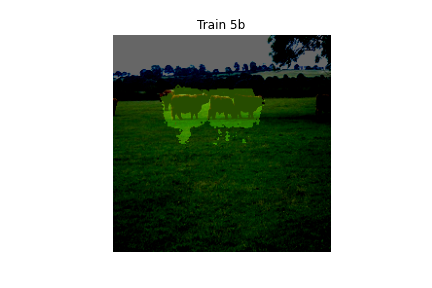
\includegraphics[width=\textwidth]{include/best model/cow1_over_actual.png} % Adjust width as needed
    \caption{Cow Over Actual Mask}
  \end{subfigure}
  \begin{subfigure}[b]{0.45\textwidth}
    \centering
    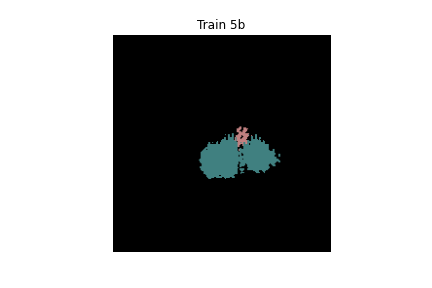
\includegraphics[width=\textwidth]{include/best model/motorbike1_pred.png}
    \caption{Motorbike Prediction Mask}
  \end{subfigure}
  \hfill %add desired spacing between images, e. g. ~, \quad, \qquad, \hfill etc. 
  %(or a blank line to force the subfigure onto a new line)
  \begin{subfigure}[b]{0.45\textwidth}
    \centering
    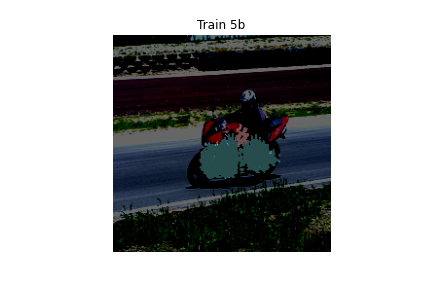
\includegraphics[width=\textwidth]{include/best model/motorbike1_over_actual.png} % Adjust width as needed
    \caption{Motorbike Over Actual Mask}
  \end{subfigure}
  \begin{subfigure}[b]{0.45\textwidth}
    \centering
    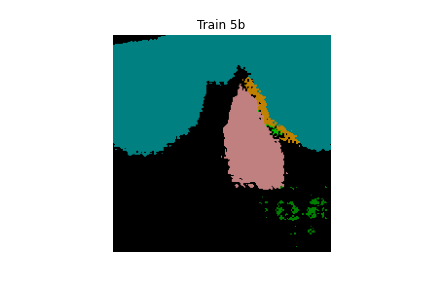
\includegraphics[width=\textwidth]{include/best model/msc1_pred.png}
    \caption{Miscelanous Prediction Mask}
  \end{subfigure}
  \hfill %add desired spacing between images, e. g. ~, \quad, \qquad, \hfill etc. 
  %(or a blank line to force the subfigure onto a new line)
  \begin{subfigure}[b]{0.45\textwidth}
    \centering
    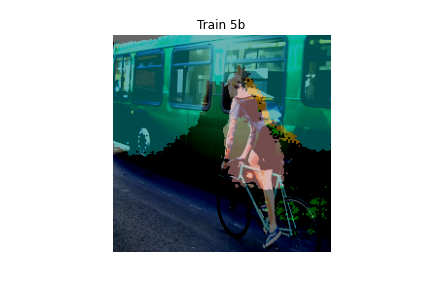
\includegraphics[width=\textwidth]{include/best model/msc1_over_actual.png} % Adjust width as needed
    \caption{Miscelanous Over Actual Mask}
  \end{subfigure}
  \begin{subfigure}[b]{0.45\textwidth}
    \centering
    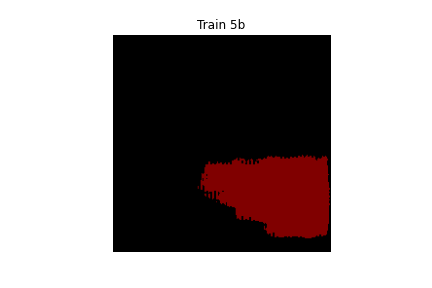
\includegraphics[width=\textwidth]{include/best model/plane1_pred.png}
    \caption{Plane Prediction Mask}
  \end{subfigure}
  \hfill %add desired spacing between images, e. g. ~, \quad, \qquad, \hfill etc. 
  %(or a blank line to force the subfigure onto a new line)
  \begin{subfigure}[b]{0.45\textwidth}
    \centering
    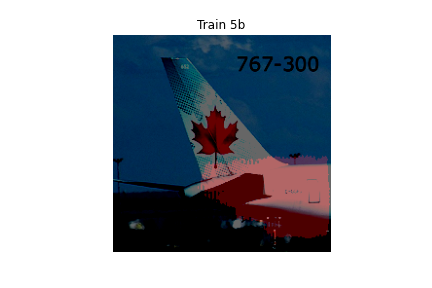
\includegraphics[width=\textwidth]{include/best model/plane1_over_actual.png} % Adjust width as needed
    \caption{Plane Over Actual Mask}
  \end{subfigure}
  \label{fig:best_models2}
\end{figure}


\newpage
\section{Contributions}

\subsection{Jack}
We all worked together for the most part of the PA, but I was in charge with Vivian for the U-net model code, and the weights imbalanced code. I also worked a lot of the report since I had the most experience with Latex, and offline, I also did a lot of debugging in my own time for our group as a world in order to make sure that the models were working correctly. E.g I found a bug in the IoU implementation that was making our best model selection incorrect.

Overall I think we all contributed equally to the project, and we all worked together to make sure that we were all on the same page and that we were all working on the same thing.


\subsection{Hou}
Hou pair-programmed with Elsie in implementing the util.py file and baseline model for train.py. He applied transformers (4b) and worked with Elsie on implementing a custom architecture and ResNet50 (5a and 5b). In the report, he wrote the Abstract, Data Augmentation, UNet, Accuracy/IoU, and created some of the tables and images shown. 

\subsection{Elsie}
Elsie pair-programmed with Hou in implementing the util.py file and baseline model for train.py. She implemented cosine annealing (4a) and worked with Hou on implementing a custom architecture and ResNet50 (5a and 5b). In the report, she wrote Cosine Annealing, ResNet50, and Q3 and Q4 subsection of the Discussion section.

\subsection{Vivian}
Vivian pair-programmed with Jack in implementing 4c and 5c and wrote the README.md. She assisted with debugging mostly the IOU function and the plot function. In the report, she wrote the Imbalanced Class Problem and Q5 of the discussion section.

%%%%%%%%%%%%%%%%%%%%%%%%%%%%%%%%%%%%%%%%%%%%%%%%%%%%%%%%%%%%%
% References/ Bibliography
%%%%%%%%%%%%%%%%%%%%%%%%%%%%%%%%%%%%%%%%%%%%%%%%%%%%%%%%%%%%%

\bibliographystyle{plainnat}
\bibliography{references}


%%%%%%%%%%%%%%%%%%%%%%%%%%%%%%%%%%%%%%%%%%%%%%%%%%%%%%%%%%%%
\appendix
\section{Appendix}
\label{sec:appendix}

\subsection{U-Net Architecture}
\label{sec:unet_architecture}
\begin{figure}
  \centering
  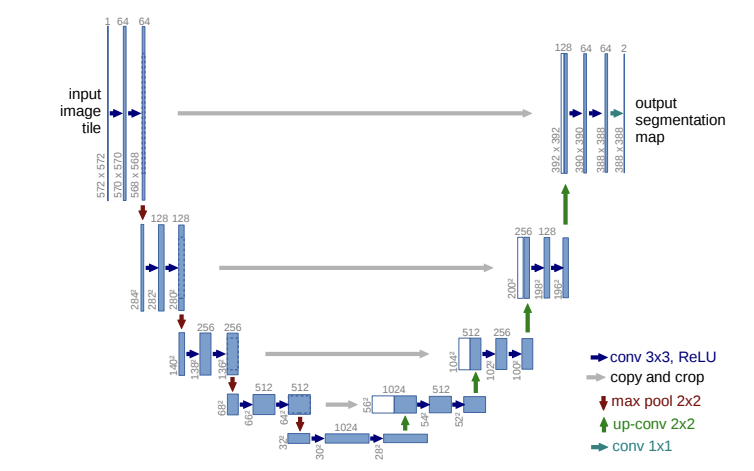
\includegraphics[width=0.8\textwidth]{include/u-net.png}
  \caption{U-Net Architecture}
  \label{fig:unet_architecture}
\end{figure}

\subsection{U-Net Crop and Copy Functionality}
\label{sec:unet_crop_copy}
\begin{minted}[autogobble]{python}
  def crop(self, source, target):
      target_size = target.size()[2:]
      source_size = source.size()[2:]

      delta = [(s - t) // 2 for s, t in zip(source_size, target_size)]
      return source[:, :, delta[0]:source_size[0] - delta[0], delta[1]:source_size[1] - delta[1]]
\end{minted}
and during the decoder, we used the crop and copy function as follows:
\begin{minted}[autogobble]{python}
  up_pool1 = self.up_pool1(bottleneck)
  if self.cropb:
      up_pool1_cropped = self.crop(conv4, up_pool1)  
      concat1 = torch.cat((up_pool1, up_pool1_cropped), 1)   

  up_conv11 = self.relu(self.bn_up_conv1(self.up_conv11(concat1)))
  up_conv1 = self.relu(self.bn_up_conv1(self.up_conv1(up_conv11)))
\end{minted}

\subsection{Weight imbalanced code}
\label{sec:weight_imbalanced_code}
\begin{minted}[autogobble]{python}
  def getClassWeights(dataset):
    """
    Calculate the class weights for a given dataset to handle class imbalance.

    Parameters:
    dataset (torch.utils.data.Dataset): The dataset containing the samples and labels.

    Returns:
    torch.Tensor: The class weights for each class in the dataset, inversely proportional to class frequencies.
    """
    class_counts = torch.zeros(21, dtype=torch.long)
    for _, label in dataset:
        label = label.long()  # Ensure label is of type torch.long for bincount
        class_counts += torch.bincount(label.view(-1), minlength=21)
    
    # Avoid division by zero for classes not present in the dataset
    class_counts[class_counts == 0] = 1
    
    total_samples = class_counts.sum().float()
    class_weights = total_samples / class_counts
    
    # Normalize weights to sum to 1, if desired (optional, depending on use case)
    class_weights /= class_weights.sum()
\end{minted}

\subsection{Data Augmentation Code}
\label{sec:data_augmentation_code}
\begin{minted}[autogobble]{python}
  class CommonTransforms:
    """
    A class that defines common image transformations.

    Args:
        size (tuple): The desired size of the transformed image. Default is (224, 224).

    """

    def __init__(self, size=(224, 224)):
        self.size = size
        self.mean_std = ([0.485, 0.456, 0.406], [0.229, 0.224, 0.225])

    def __call__(self, img, mask):
        """
        Applies common image transformations to the input image and mask.

        Args:
            img (PIL.Image.Image): The input image.
            mask (PIL.Image.Image): The input mask.

        Returns:
            tuple: A tuple containing the transformed image and mask.

        """
        # Random horizontal flip with the same decision for both img and mask
        if random.random() > 0.5:
            img = F.hflip(img)
            mask = F.hflip(mask)

        # Random resized crop with the same parameters for both img and mask
        i, j, h, w = transforms.RandomResizedCrop.get_params(img, scale=(0.08, 1.0), ratio=(3./4., 4./3.))
        img = F.resized_crop(img, i, j, h, w, self.size, InterpolationMode.BILINEAR)
        mask = F.resized_crop(mask, i, j, h, w, self.size, InterpolationMode.NEAREST)

        # Convert images to tensors without normalization
        img = standard_transforms.functional.to_tensor(img)
        # Normalize image using mean and standard deviation
        img = standard_transforms.functional.normalize(img, *self.mean_std)

        # Convert mask to tensor with long dtype and handle values of 255
        mask = torch.as_tensor(np.array(mask), dtype=torch.long)
        mask[mask == 255] = 0

        return img, mask
\end{minted}
\end{document}